\chapter{Implementierung}

Die Implementierung wird in zwei Teile gegliedert, Learning Management System (LMS) und WebVR Applikation. Bei dem Teil LMS werden die Auswahl von LMS und die Erstellung des Unterrichts über die Vorbereitung einer Infusion thematisiert. Bei dem Teil WebVR Applikation werden von Auswahl des Frameworks bis Implementierungen der Features, die beim Kapitel Konzeption gestaltet sind, erklärt.

\section{Learning Managment System}

Viele LMS werden auf dem Markt angeboten. Eine geeignete Plattform für das Projekt wird ausgewählt, worauf ein Unterricht zur Infusionsvorbereitung gestaltet wird. ein paar Lernmethoden, beispielsweise VR Übungen, werden im Unterricht eingesetzt.

 \subsection{LMS Auswahl}

 Laut Capterra stehen mehr als 400 LMS mit Web Applikation zu Verfügung. Jedes LMS hat eigene Merkmale. Moodle ist ein LMS auf dem Markt, dessen Eigenschaften gut zu diesem Projekt passen.
 
 Der größte Vorteil von Moodle für das Projekt ist, dass Moodle eine kostenlose open source LMS Plattform ist. Das heißt, dass es möglich ist, Moodle gratis auf den eigenen Server zu installieren, mit einer eigenen Datenbank zu verbinden und nach eigenen Anforderungen einzustellen.
 
 In Moodle können auch Arbeitsmaterialien wie Bücher, Dateien, Links usw. angeboten werden. Bei diesem Projekt wird der Nutzer durch den URLs in Moodle zu der WebVR Applikation geleitet, wie die erste Form, die in dem Kapitel Konzeption beschrieben wird. 
 
 \subsection{Unterricht}
 Bei dem Unterricht zur Infusionsvorbereitung werden fünf Arbeitsmaterialien (drei Links, eine Datei und ein Textseite) und eine Aktivität eingesetzt. Die drei Links leiten jeweils auf einer Erklärung zur Infusionsvorbereitung in Text, einer Erzählung über 5-R-Regel in Text und einem Video über Infusionsvorbereitung auf Youtube um. Die Datei ist ein Diagramm, damit der Ablauf der Vorbereitung einer Infusion graphisch dargestellt wird.
 
 Die Textseite bietet den Zugang der praktischen Übung in VR Umgebung. Über die Methoden der Interaktion für unterschiedliche Geräten wird zuerst informiert. Danach wird der Ablauf mit dem Diagramm noch einmal wiederholt. Und die acht Abschnitte in der Übung werden bezeichnet. Zum Abschluss werden acht Links aufgelistet, die auf dem entsprechenden Abschnitt in der VR Übung umleiten.
 
 Am Ende des Unterrichtes wird die Aktivität Test angeboten. Dadurch wird der Lerneffekt überprüft. Und das Ergebnis wird in Moodle gespeichert.
 
 Die VR Übung und der Test sind wiederholbar, um den Lernenden zu helfen, die Fertigkeit richtig zu beherrschen.
 
 image: Unterricht und Textseite ......... bis fertig von Unterricht
 
\section{WebVR Applikation}
Die Implementierung der WebVR Applikation ist der Schwerpunkt dieses Projektes. Im ersten Teil werden die Realisierungen, die das ganze Projekt betreffen, thematisiert, danach werden die Implementierungen der kleinen Features erklärt.

 \subsection{Framework Auswahl}
 
 Um die gesetzten Ziele dieses Projektes zu erreichen, muss das ausgewählte Framework folgende Anforderungen erfüllen:
 
 \begin{enumerate}
     \item Das Projekt kann gut mit LMS kommunizieren. Die Kommunikation kann durch URL oder Datenbank realisiert werden.
     \item Das Framework kann unterschiedliche Geräte unterstützen, z.B. PC, Smartphone und HMD.
     \item Das Projekt kann auf einem eigenen Server bewahrt werden.
     \item Die Nutzung ist kostenlos.
     \item Reichliche Dokumentation und erreichbare Community stehen zu Verfügung.
     \item Das Framework soll lange Zeit unterstützt und am besten kontinuierlich weiterentwickelt werden.
 \end{enumerate}
 
 Im Kapitel Stand der Technik wird die Technologie der WebVR vorgestellt. Fünf Frameworks und Game Engines davon sind in der Lage, WebVR Applikation effizient zu entwickeln, nämlich Unity, Play Canvas, Vizor, React 360 und A-Frame.
 
 \begin{itemize}
 
     \item \textbf{Unity} \citep{37} ist ein umfangreiche Game Engine. Viele built-in Funktionen stehen zu Verfügung. Mit dem Plugin von Mozilla kann ein Projekt als WebVR Applikation exportiert werden. Allerdings wird das Projekt in einen Rahmen gestellt. In diesem Rahmen ist die Entwicklung hoch effizient. Aber es ist schwierig, mit den Dinge außerhalb des Rahmens, beispielsweise LMS, anzupassen. Deswegen wird Unity nicht ausgewählt.
     
     \item \textbf{Play Canvas} \citep{38} ist eine webbasiert Game Engine. Damit kann das Projekt direkt als WebVR Applikation exportiert werden. Aber wenn man die Applikation auf einem eigenen Server bewahren möchte, muss man monatlich zahlen. (Abbildung ~\ref{fig:Webbasierte Engine})
     
     \item \textbf{Vizor} \citep{39} ist eine webbasierte visuelle WebVR Plattform. Die Scripts werden durch Blueprints geschrieben. Ihre Stärke ist, die 360 Grad oder VR Szene darzustellen. Allerdings reicht die Unterstützung für Interaktion für dieses Projekt nicht aus. (Abbildung ~\ref{fig:Webbasierte Engine})
     
     \item \textbf{React 360} \citep{40} basiert teilweise auf three.js und wird von Facebook entwickelt. Die Logik der Entwicklung von React 360 ist die gleiche wie die bekannte JavaScript Bibliothek React im Bereich Frontend-Entwicklung. Allerdings wurde React 360 noch nicht vorgestellt, als dieses Projekt anfing. Damals existierte nur der Vorfahre von React 360, nämlich React VR. Aber die Funktionalität von React VR war nicht ausreichend genug, dieses Projekt zu entwickeln.
     
     \item \textbf{A-Frame} \citep{41} ist ein von Mozilla entwickeltes kostenloses open source WebVR Framework. Es bietet die größte Freiheit, das Projekt zu manipulieren. Außerdem werden unterschiedliche Geräte unterstützt. Mit A-Frame werden die Funktionen von three.js in einem Entity-Component System eingewickelt. Die Features von three.js werden vererbt. Die Lösungen der Probleme über die Entwicklung können entweder in der Community von A-Frame oder der Community von three.js gefunden werden.
     
 \end{itemize}
 
\begin{figure}[ht]
\centering
\caption[Webbasierte Engine]{Webbasierte Editoren von PlayCanvas \& Vizor}
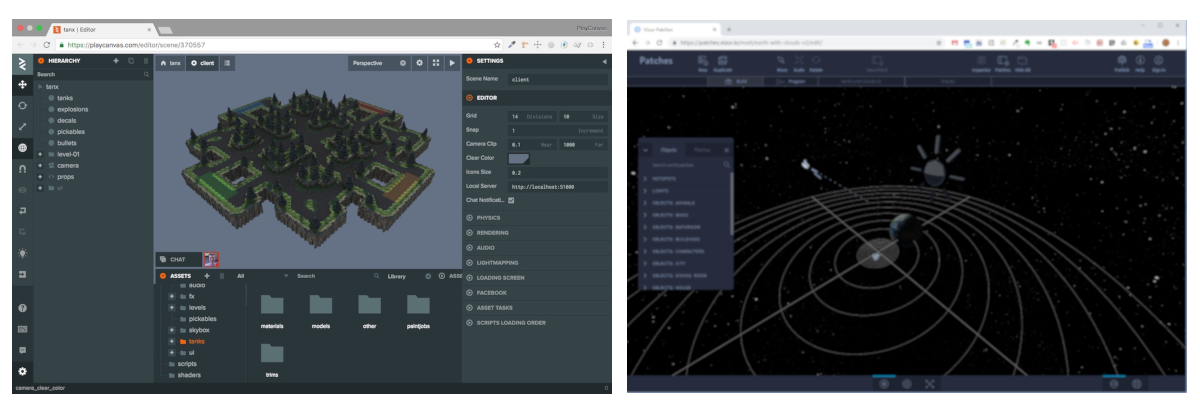
\includegraphics[width=\textwidth]{images/playCanvasVizor.png}
\label{fig:Webbasierte Engine}
\end{figure}

 A-Frame kann alle Anforderungen erfüllen. Deshalb fällt die Entscheidung nach dem Vergleich auf A-Frame.
 
 \subsection{Projektierung}
 Im Bereich Web Entwicklung werden zwei beliebte Werkzeuge geboten, Node Package Manager (npm) und Webpack. Mit den Beiden Werkzeugen kann Web Applikation projektiert werden und die Effizient der Entwicklung gefördert werden.
 
 Npm ist ein Packetmanager für die JavaScript-Laufzeitumgebung Node.js. Mit npm ist es einfach, die auf npm gespeicherten Pakete (Software) zu benutzen. Die Abhängigkeit der Pakete wird durch npm automatisch behandelt. Alle benutzten Pakete werden in einer Datei eingepackt, sodass der Einsatz auf dem Server erleichtert wird. (Abbildung ~\ref{fig:npmWebpack})
 
 Webpack ist ein auf npm gespeichertes Werkzeug, das verwendete und geschriebene Dateien organisiert. Während der Entwicklung einer Web Applikation werden vielen Dateien beispielsweise Javascript Dateien, HTML Dateien, CSS Dateien, Bilder usw. benutzt. Die Dateien sind getrennt, aber mit einander verbunden. Solch eine dezentralisierte Struktur führt zum hohen Aufwand, das Projekt auf einem Server zu bewahren. Durch Webpack werden die Dateien während der Entwicklung bündig verpackt und komprimiert. (Abbildung ~\ref{fig:npmWebpack})
 
\begin{figure}[ht]
\centering
\caption[Projektierungswerkzeuge]{npm \& Webpack}
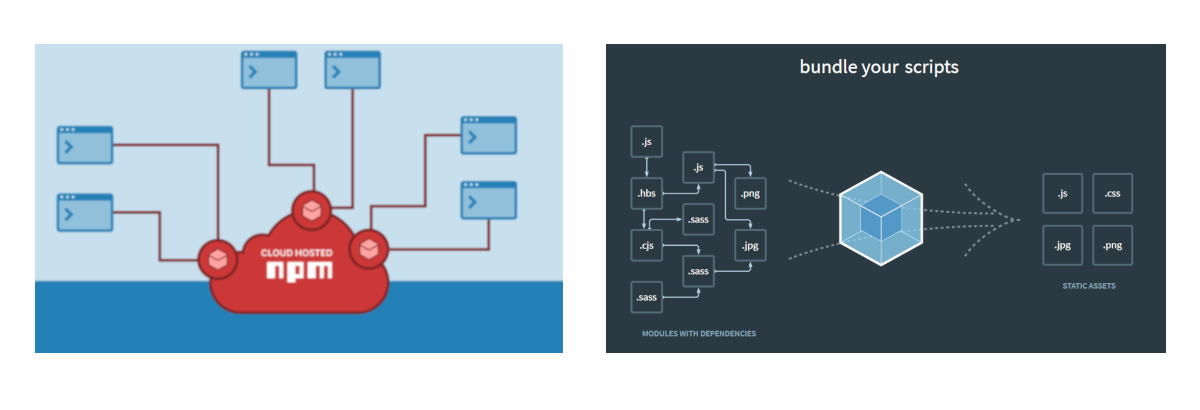
\includegraphics[width=\textwidth]{images/npmWebpack.png}
\label{fig:npmWebpack}
\end{figure}
 
 Webpack-dev-server ist ein zusätzliches Werkzeug von Webpack. Dadurch werden die verpackten JavaScript Dateien automatisch kompiliert und die Webseite im Browser automatisch aktualisiert, solange die Codes geändert werden.
 
 Während der Entwicklung einer Web Applikation können die CORS (Cross-Origin Resource Sharing) Errors auftauchen, wenn die lokale zugängliche Datei direkt im Browser aufgerufen wird, um den Effekt im Code anzuschauen. Der Grund ist, dass zur Sicherheit die Browsers Same-Origin-Policy (Abbildung ~\ref{fig:Same-Origin-Policy}) benutzt werden. Das heißt, dass es untersagt wird, auf Objekte (zum Beispiel Grafiken) zuzugreifen, die von einer anderen Webseite stammen oder deren Speicherort nicht der Origin entspricht. Die vom Browser direkt aufgerufenen lokalen Dateien gelten nicht als Same-Origin requests sondern als Cross-Origin requests.
 
\begin{figure}[ht]
\centering
\caption[Same-Origin-Policy]{Same-Origin-Policy}
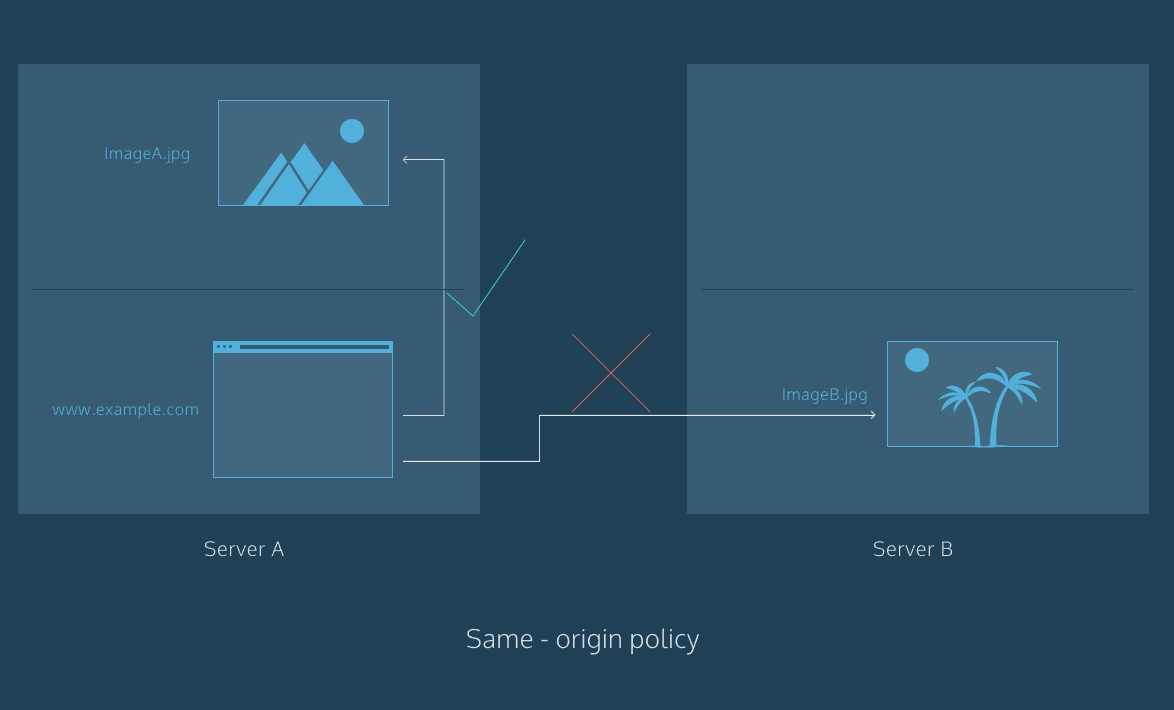
\includegraphics[width=\textwidth]{images/sameOrigin.png}
\label{fig:Same-Origin-Policy}
\end{figure}
 
 Http-server ist ein auf npm gespeichertes Werkzeug, wodurch ein Server (localhost) auf einem eigenen PC erstellt werden kann. Und ein ausgewählter Ordner auf dem PC wird als das Wurzelverzeichnis des Servers eingerichtet. Alle Dateien in diesem Ordner gelten als in dem gleichen Origin, sodass die CORS Errors behoben werden.
 
 Nach der Projektierung ist die Struktur der Applikation wie in Abbildung ~\ref{fig:projektStruktur} gezeigt wird.
 
\begin{figure}[ht]
\centering
\caption[Struktur des Projekts]{Struktur des Projekts}
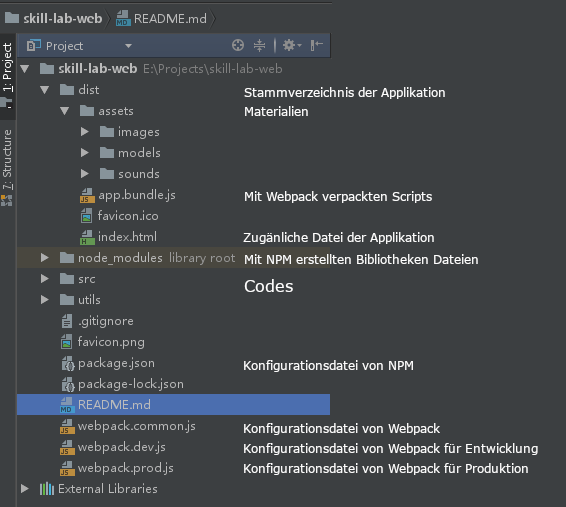
\includegraphics[width=\textwidth]{images/projektSturktur.png}
\label{fig:projektStruktur} 
\end{figure}
 
 \subsection{Zustände Management für Fortschritte}
 Im Kapitel Konzeption werden die Erkennung und Feedback Fortschritte thematisiert. In diesem Kapitel wird erklärt, wie die Fortschritte in der Applikation implementiert werden.
 
 Um die Fortschritte zu definieren, wird die Konzeption \glqq state container\grqq von der Technik Redux importiert. Jedes Objekt in der VR Szene hat einen eigenen Zustand, zum Beispiel Position. Die betreffenden Zustände werden geändert, wenn der Prozess der Applikation betrieben wird. Die Sammlung der Zustände der ganzen Objekten wird als \glqq state container\grqq bezeichnet. Durch die Kombination der Zustände wird der Fortschritt der Übung notiert.
 
 Wenn eine Aktivität auf dem Objekt durchgeführt wird, wird zuerst die Interaktion auf einem Objekt erkannt. Danach werden die betroffenen Zustände geändert. Laut der Änderung der Zustände wird die entsprechende Aktivität des Objektes durchgeführt, was als Feedback an dem Benutzer geht. (Abbildung ~\ref{fig:interaktionVerlauf})
 
\begin{figure}[ht]
\centering
\caption[Durchlauf einer Aktivität]{Durchlauf einer Aktivität}
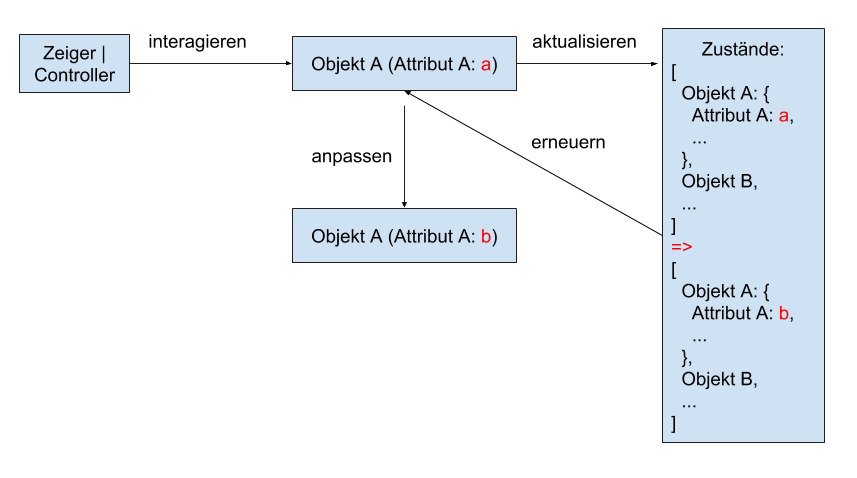
\includegraphics[width=\textwidth]{images/interaktionVerlauf.png}
\label{fig:interaktionVerlauf} 
\end{figure}
 
  \subsubsection{Beobachter (en. Observer Pattern)}
  Beobachter ist ein Entwurfsmuster (en. Design Pattern) aus dem Bereich Softwareentwicklung. Es ist dafür geeignet, um das Zustandsmanagement zu implementieren.
  
  %TODO: ist es so richtig(Zum Beispiel von Linus Torvalds)? (von Le)
  Die Funktionalität davon ist ähnlich wie der Mechanismus von Twitter. Zum Beispiel Linus Torvalds \citep{42} von der Socialmediaplattform Twitter, die es seit 2012 gibt und wo Nutzer einen Account anlegen und anderen Nutzern \glqq folgen \grqq\ können. Bei Posts einer gefolgten Person werden die \glqq Folgenden \grqq\ benachrichtigt. (Abbildung ~\ref{fig:observerPatern})
  
  Im Bereich Softwareentwicklung wird der Gefolgten als \glqq Observable\grqq oder \glqq Subject\grqq bezeichnet. Die Folgenden werden als \glqq Observer\grqq bezeichnet. Die Aktivität \glqq follow\grqq ist \glqq Subscribe\grqq. Die Benachrichtigung heißt \glqq Notify\grqq.
  
\begin{figure}[ht]
\centering
\caption[Observer Pattern]{Observer Pattern}
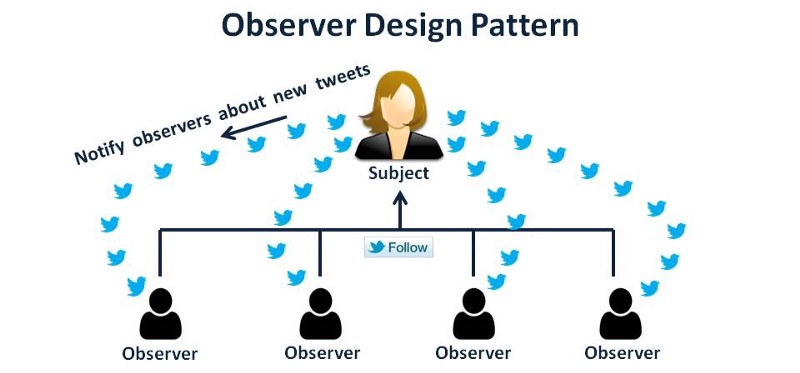
\includegraphics[width=\textwidth]{images/observerPattern.jpeg}
\label{fig:observerPatern} 
\end{figure}
  
  Um das Oberserver Pattern zu implementieren, wird eine Klasse {\fontfamily{qcr}\selectfont Observable} in diesem Projekt erstellt. (Abbildung ~\ref{fig:observable})
  
\begin{figure}[ht]
\vspace*{1em}
\centering
\caption[Class Observable]{Class Observable}
%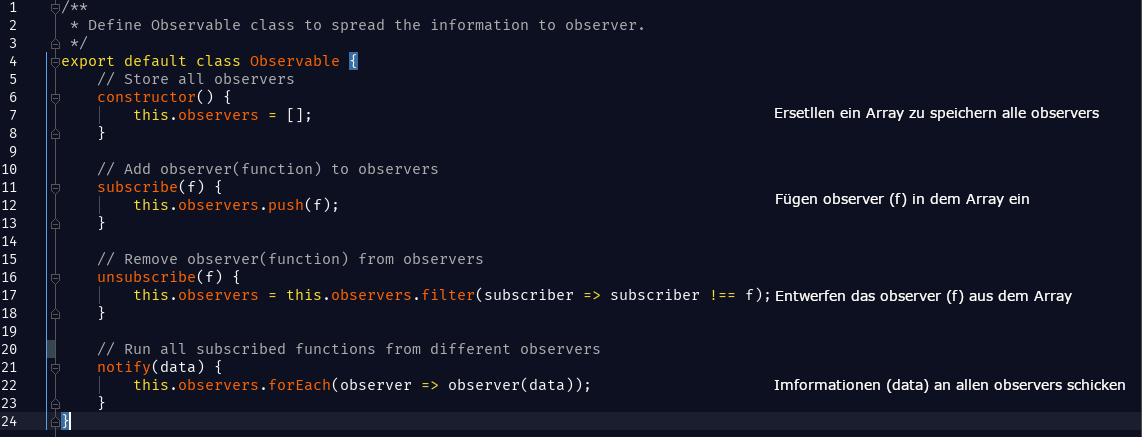
\includegraphics[width=\textwidth]{images/observable.png}
\begin{lstlisting}[language=JavaScript, style=htmlcssjs]
export default class Observable {
    // Store all observers
    constructor() {
        this.observers = [];
    }
    // Add observer(function) to observers
    subscribe(f) {
        this.observers.push(f);
    }
    // Remove observer(function) from observers
    unsubscribe(f) {
        this.observers = this.observers.filter(subscriber => subscriber !== f);
    }
    // Run all subscribed functions from different observer
    notify(data) {
        this.observers.forEach(observer => observer(data));
    }
}
\end{lstlisting}
\label{fig:observable} 
\end{figure}
  Während der Erstellung einer Instanz von {\fontfamily{qcr}\selectfont Observable} wird ein Array {\fontfamily{qcr}\selectfont Observers} generiert, um die Funktionen von \glqq Observers\grqq\ zu speichern. Durch die Funktionen {\fontfamily{qcr}\selectfont subscribe} und {\fontfamily{qcr}\selectfont unsubscribe} können die Funktionen von \glqq Observer\grqq\ in dem Array eingefügt oder von dem Array ausgezogen werden. Die \glqq Observers\grqq\ sollen eine Funktion mit einem Parameter haben, um die Nachrichten von {\fontfamily{qcr}\selectfont Observable} zu empfangen. Wenn die Funktion {\fontfamily{qcr}\selectfont Notify} aufgerufen wird, werden alle abonnierten Funktionen von \glqq Observers\grqq\ in dem Array {\fontfamily{qcr}\selectfont Observers} nacheinander aufgerufen. Der Parameter der Funktion {\fontfamily{qcr}\selectfont Notify} wird als Parameter der Funktion von \glqq Observers\grqq\ eingesetzt, sodass die Nachrichten ausgeteilt werden.
  
  \subsubsection{Zustände Management}
  
  Um das Zustandsmanagement zu realisieren, wird ein Klasse {\fontfamily{qcr}\selectfont stateIndex} geschrieben. Da fast alle Objekt in der Szene mit dieser Klasse verbunden sind und den einzigen \glqq state container\grqq referenzieren, wird die Klasse als \glqq static\grqq Klasse definiert.
  
  %TODO: ist es so richtig(static zu erklären)? (von Le)
  Die \glqq static\grqq\ Klasse hat keine Entität. Die zugehörigen Funktionen werden direkt durch die Klasse aufgerufen. Da es kein \glqq static\grqq\ Klasse in JavaScript gibt, gilt die Klasse, deren allen zugehörigen Attributen und Funktionen \glqq static\grqq\ sind, als \glqq static\grqq Klasse.
  
  Mit der Funktion {\fontfamily{qcr}\selectfont init}  werden alle Zustände initialisiert. Die Initialisierung liegt an dem Query string in URL (Abbildung ~\ref{fig:queryString}). Der Query string ist ein Teil von URL, wodurch der Parameter bei dem \glqq request\grqq zusammen an den Server geschickt wird. Bei dieser Applikation ist der Query string die Ziffer des ausgewählten Abschnitts. Mit dem Query string werden die Zustände nach dem ausgewählten Abschnitt initialisiert.
  
  Während der Initialisierung wird eine Entität von {\fontfamily{qcr}\selectfont Observable} erstellt, um die Benachrichtigung zu verbreiten.
  
  Die {\fontfamily{qcr}\selectfont init} Funktion wird nur einmal aufgerufen, wenn die Applikation aufgerufen wird.
  
\begin{figure}[ht]
\centering
\caption[Query String]{Query String}
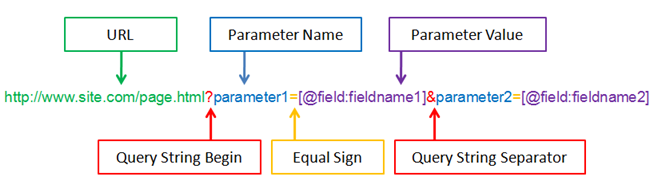
\includegraphics[width=\textwidth]{images/queryString.png}
\label{fig:queryString} 
\end{figure}
  
  Zu Sicherheit dürfen die Zustände von anderen Objekt nicht erreichbar sein. Deswegen werden die Funktionen von der Klasse {\fontfamily{qcr}\selectfont stateIndex} angeboten, um die Zustände zu manipulieren.
  
  \begin{itemize}
      \item {\fontfamily{qcr}\selectfont getState}: um alle aktuelle Zustände zu bekommen.
      \item {\fontfamily{qcr}\selectfont get}: um einen bestimmte Zustand zu bekommen.
      \item {\fontfamily{qcr}\selectfont getIn}: um einen bestimmten Zustand in tiefen Ebenen zu bekommen.
      \item {\fontfamily{qcr}\selectfont set}: um einen bestimmten Zustand zu aktualisieren. Durch die Funktion {\fontfamily{qcr}\selectfont Notify} von \glqq Observable\grqq\ werden neue Zustände an alle \glqq Observer\grqq\ geschickt.
      \item {\fontfamily{qcr}\selectfont setIn}: um einen bestimmten Zustand in tiefen Ebenen zu aktualisieren. Durch der Funktion {\fontfamily{qcr}\selectfont Notify} von \glqq Observable\grqq\ werden die neuen Zustände an alle \glqq Observer\grqq\ ausgeteilt.
  \end{itemize}
  
 \subsection{Abschnitte Auswahl}
 Die Auswahl der Abschnitte kann zu zwei Zeitpunkten durchgeführt werden. Einer davon ist während des Aufrufs der Applikation. Die Ziffer des ausgewählten Abschnitts wird durch den Query string in URL an die Applikation weitergegeben. Der andere Zeitpunkt ist vor dem Nehmen der Krankenakte in der VR Szene. Auf dem Whiteboard werden die Abschnitte aufgelistet, wodurch ein bestimmter Abschnitt ausgewählt werden kann.
 
  \subsubsection{Abschnitte Auswahl durch URL}
  Die Zustände werden am Anfang als ursprüngliche Zustände initialisiert. Durch die Funktion {\fontfamily{qcr}\selectfont getSectionSelectionFromURL} in der Klasse {\fontfamily{qcr}\selectfont stateIndex} kann die ausgewählte Ziffer bestimmt werden. Wenn die Ziffer zwischen 1 und 7 ist, werden die betroffenen Zustände durch die Funktion {\fontfamily{qcr}\selectfont selectSection} aktualisiert. Danach werden die Objekte in der Szene nach den Zuständen auch aktualisiert.
  
  Um die GUI richtig einzusetzen, wird ein Trick benutzt. Wenn die Applikation aufgerufen wird, wird die Szene nach den aktuellen Zuständen eingerichtet und es werden gleichzeitig die Modelle geladen. Es könnte passieren, dass ein Modell noch nicht fertig geladen ist, wenn es von der Aktualisierung betroffen ist. Das führt zu Fehlern in der Applikation.
  
  Um das Problem zu lösen, wird die Ladung vor der Aktualisierung überprüft (Abbildung ~\ref{fig:checkLadung}). Mit der Funktion {\fontfamily{qcr}\selectfont setInterval} wird es implementiert, alle 0,5 Sekunden den Zustand der Ladung zu überprüfen. Wenn alle Modelle schon geladen sind, wird die Überprüfung beendet und die Szene aktualisiert.
  
\begin{figure}[ht]
\vspace*{1.2em}
\centering
\caption[Überprüfung der Zustände der Ladungen]{Überprüfung der Zustände der Ladungen}
%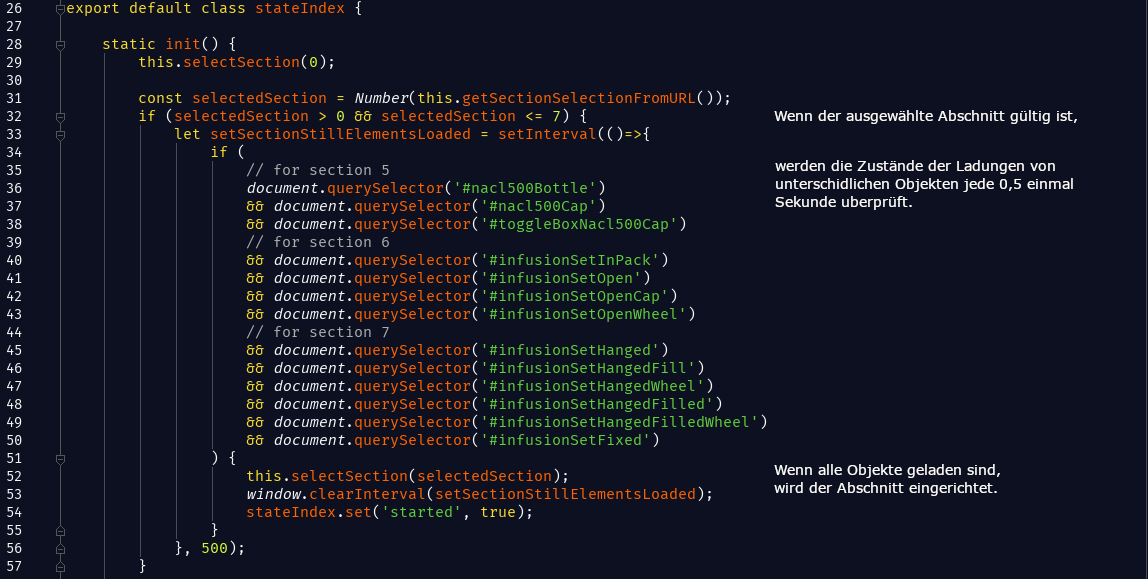
\includegraphics[width=\textwidth]{images/checkLadung.png}
\begin{lstlisting}[language=JavaScript, style=htmlcssjs]
export default class stateIndex {
    static init() {
        this.selectSection(0);
        const selectedSection = Number(this.getSectionSelectionFromURL());
        if (selectedSection > 0 && selectedSection <= 7) {
            // If selected with URL, check the staus of loading every 0.5 sec
            let setSectionStillElementsLoaded = setInterval(()=>{
                if (
                    document.querySelector('#nacl500Bottle')
                    && document.querySelector('#nacl500Cap')
                    && // other objects
                ) {
                    this.selectSection(selectedSection);
                    window.clearInterval(setSectionStillElementsLoaded);
                    stateIndex.set('started', true);
                }
            }, 500);
        }
\end{lstlisting}

\label{fig:checkLadung} 
\end{figure}
  
  \subsubsection{Abschnitte Auswahl in VR Szene}
  Auf dem Whiteboard werden die Abschnitte aufgelistet. Durch Zeiger oder Raycaster wird die Funktion {\fontfamily{qcr}\selectfont selectSection} in der Klasse {\fontfamily{qcr}\selectfont stateIndex} mit entsprechendem Parameter aufgerufen, um den Abschnitt zu wechseln.
  
  Vor den Zeichnen auf dem Whitebard werden 7 \glqq toggle boxes\grqq eingesetzt, wodurch die Funktion {\fontfamily{qcr}\selectfont selectSection} durch HTC Vive Controllers aufgerufen werden kann. (Abbildung ~\ref{fig:toggleBoxAbschnitte})
  
\begin{figure}[ht]
\vspace*{1em}
\centering
\caption[Toggle Boxes]{Toggle Boxes für die Auswahl der Abschnitte}
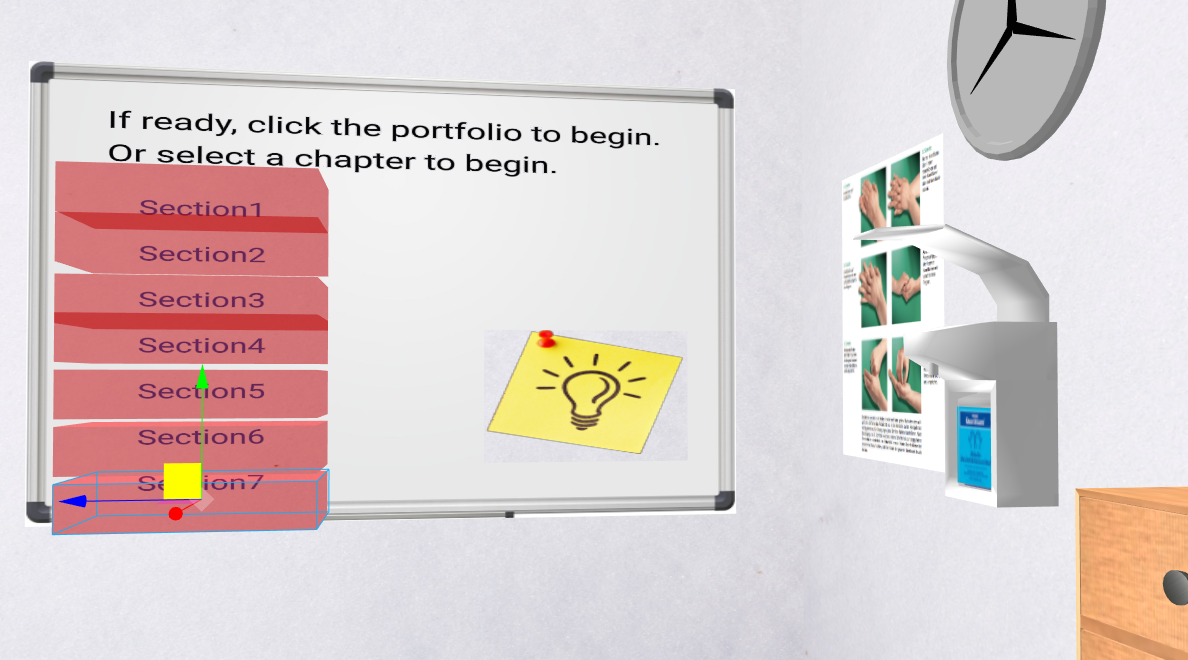
\includegraphics[width=\textwidth]{images/toggleBoxAbschnitte.png}
\label{fig:toggleBoxAbschnitte} 
\end{figure}
  
  \subsubsection{Möglichkeit der Verbesserung}
  Die Abschnitte-Auswahl kann nicht nur während der Initialisierung, sondern auch nach der Initialisierung durchgeführt wird. Deswegen sollen die Funktionen der Abschnitte-Auswahl wie {\fontfamily{qcr}\selectfont selectSection} nicht in der Klasse {\fontfamily{qcr}\selectfont stateIndex} eingepackt werden, sondern in eine eigene Datei geschrieben werden.
  
 \subsection{Gestaltung der Struktur der Klassen der Objekte}
 Um das Projekt effizient zu entwickeln, wird eine Struktur der Klassen gestaltet, die sich an die meisten Objekte in diesem Projekt anpassen kann. Die Struktur basiert auf der Klasse Struktur von A-Frame.
 
 \subsubsection{Gestaltung}
 Die Philosophie von A-Frame ist, mit spezifischen HTML Elementen die Szene aufzubauen. Ein Element ist eine Kombination der Entitäten von unterschiedlichen Klassen (Abbildung ~\ref{fig:aframeClass}). Eine Entität kann ein HTML Element oder ein Attribut eines HTML Elements sein. Das Klasse in A-Frame wird als Component bezeichnet.
 
 Drei built-in Objekte von Component sind wichtig.
 \begin{itemize}
     \item {\fontfamily{qcr}\selectfont init} ist eine Funktion, die während der Erstellung einer Entität von Component durchgeführt wird.
     \item {\fontfamily{qcr}\selectfont schema} ist ein JavaScript Objekt, das Attribute von Component speichert.
     \item {\fontfamily{qcr}\selectfont update} ist eine Funktion, die durchgeführt wird, wenn das schema durch HTML geändert wird. Die Initialisierung gilt als eine Änderung von schema, d.h. dass die Funktion update während der Erstellung einer Entität durchgeführt wird. Deswegen muss die Funktion init nicht definiert sein, wenn die Funktion update existiert.
 \end{itemize}
 
\begin{figure}[ht]
\vspace*{1em}
\centering
\caption[Typisches A-Frame Class]{typisches A-Frame Class}
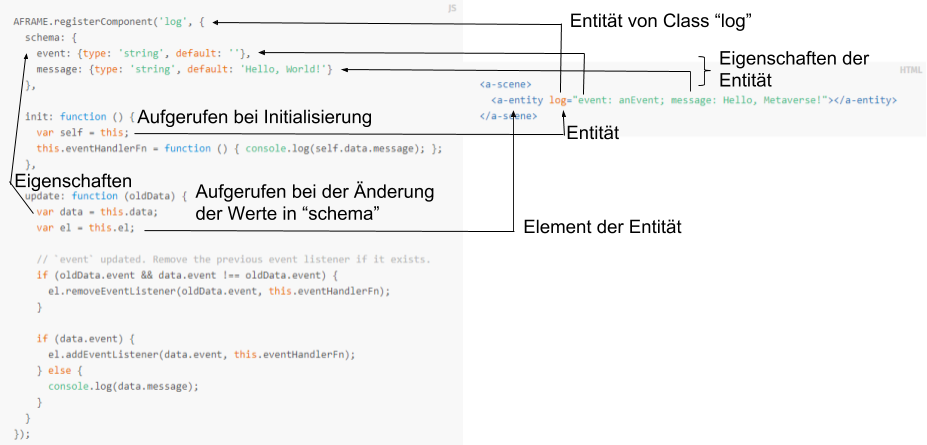
\includegraphics[width=\textwidth]{images/aframeClass.png}
\label{fig:aframeClass} 
\end{figure}
 
 Der Vorteil einer solchen Struktur ist, dass jede Entität eine eigene Kopie der Funktionen und Attribute von Component hat. Das bedeutet, dass ein Component (Klasse) viele Entitäten haben kann. Die Entitäten beeinflussen sich nicht untereinander.
 
 Allerdings muss die Struktur von Component wegen der Nutzung von Observer Pattern neu gestaltet werden.
 
 Der Code der Klasse {\fontfamily{qcr}\selectfont Observable} hat gezeigt, dass die Parameter der Funktion {\fontfamily{qcr}\selectfont subscribe} eine Funktion sein sollen. Aber die Funktionen, die in der Klasse definiert werden, gelten nicht als eine bestimmte Funktion bei JavaScript. Deshalb müssen die Funktionen, die als \glqq observer\grqq benutzt werden, außerhalb der Klasse definiert werden, sodass die Entitäten der Klasse die Nachrichten von \glqq observable\grqq\ empfangen können. Das führt zu einer suboptimalen Situation, dass alle Entität, die durch die gleiche Klasse erstellt werden, dieselben Funktionen und Eigenschaften benutzen. (Abbildung ~\ref{fig:eigenesClass})
 
 Obwohl die Struktur der Klasse sich der Philosophie von A-Frame nicht anpasst, ist es praktisch und geeignet für dieses Projekt, weil fast alle Klassen nur eine einzige Entität in der Szene haben.
 
 Um die Attribute und Funktionen von Component von die Funktion in \glqq observer\grqq\ zu erreichen, werden die Attribute und Funktionen beispielsweise {\fontfamily{qcr}\selectfont schema} auch außerhalb der Klasse als globale Variablen geschrieben.
 
\begin{figure}[ht]
\vspace*{1em}
\centering
\caption[Eigene Klassen Struktur]{Eigene Klassen Struktur}
%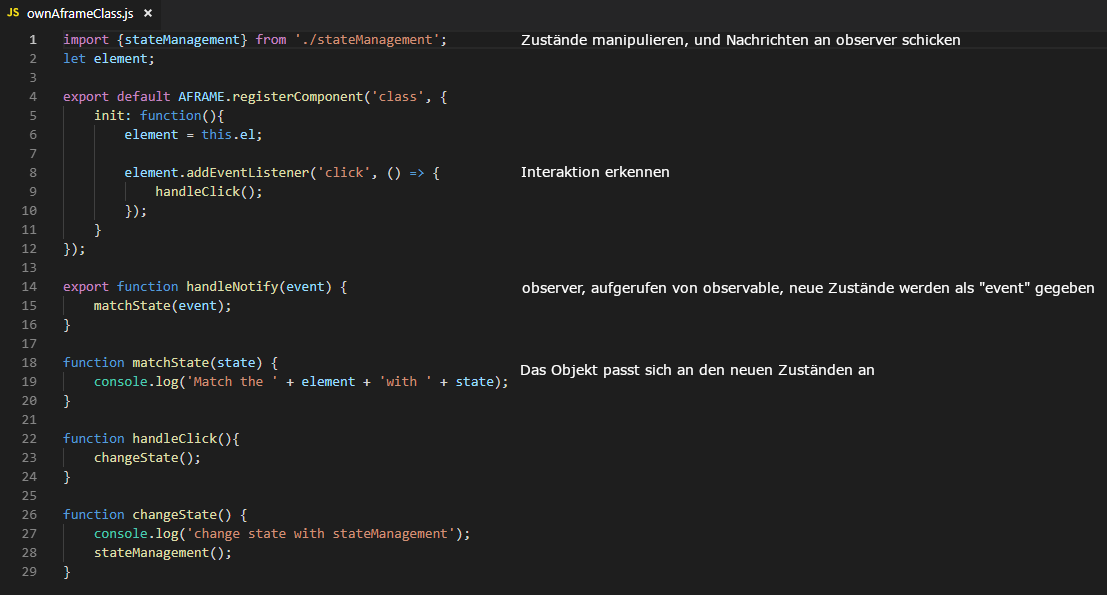
\includegraphics[width=\textwidth]{images/eigenesClass.png}
\begin{lstlisting}[language=JavaScript, style=htmlcssjs]
import {stateManagement} from './stateManagement';
let element;
export default AFRAME.registerComponent('class', {
    init: function(){
        element = this.el;
        element.addEventListener('click', () => {
            handleClick();
        });
    }
});
export function handleNotify(event) {
    matchState(event);
}
function matchState(state) {
    // match the element with its state
}
function handleClick(){
    changeState();
}
function changeState() {
    // change state with stateManagement
    stateManagement();
}
\end{lstlisting}
\label{fig:eigenesClass} 
\end{figure}
 
 \subsubsection{Möglichkeit der Verbesserung}
 Es ist auch möglich, nach der Philosophie von A-Frame die Klassen Struktur zu gestalten.
 
 Durch anpassen von {\fontfamily{qcr}\selectfont addEventListener} ({\fontfamily{qcr}\selectfont on} in Jquery), das während der Initialisierung eingefügt wird, kann die Nachricht von \glqq observable\grqq\ in die Klasse transportiert werden. (Abbildung ~\ref{fig:bestesClass})
 
\begin{figure}[ht]
\vspace*{1em}
\centering
\caption[Bessere Klassen Struktur]{Bessere Klassen Struktur}
%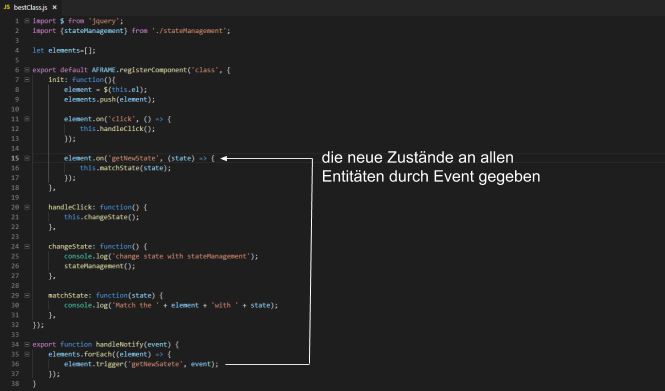
\includegraphics[width=\textwidth]{images/bestClass.png}
\begin{lstlisting}[language=JavaScript, style=htmlcssjs]
import $ from 'jquery';
import {stateManagement} from './stateManagement';
let elements=[];
export default AFRAME.registerComponent('class', {
    init: function(){
        element = $(this.el);
        elements.push(element);
        element.on('click', () => {
            this.handleClick();
        });
        // emitted by handleNotify()
        element.on('getNewState', (state) => {
            this.matchState(state);
        });
    },
    handleClick: function() {
        this.changeState();
    },
    changeState: function() {
        // change state with stateManagement
        stateManagement();
    },
    matchState: function(state) {
        // match the element with its state
    },
});
export function handleNotify(event) {
    elements.forEach((element) => {
        element.trigger('getNewSatete', event);
    });
}
\end{lstlisting}
\label{fig:bestesClass} 
\end{figure}
 
 \subsection{Interaktion}
  Für unterschiedliche Geräte werden entsprechende Interaktionen konzipiert. Die Implementierungen werden der Reihe nach je nach Gerät aufgelistet.
  
  \subsubsection{PC und Smartphone}
  Viele Interaktionen auf dem PC und Smartphone werden durch dasselbe Component umgesetzt, deswegen werden die Implementierung von PC und Smartphone zusammen erklärt.
  
  \vspace{1em}
  \noindent
  \textbf{Exploration}
  \vspace{1em}
  
  \noindent
  Mit einer Entität von built-in Component {\fontfamily{qcr}\selectfont a-camera} in A-Frame wird eine Kamera in der Szene eingesetzt (Abbildung ~\ref{fig:cameraHtml}). Dadurch wird die Sicht des Nutzers in der VR Umgebung erstellt. Die Interaktionen, die die Kamera betreffen, nämlich Exploration und Navigation werden in dieser Entität realisiert.
  
  Mit dem Component {\fontfamily{qcr}\selectfont look-controls} kann die Rotation einer Entität manipuliert werden. Wenn {\fontfamily{qcr}\selectfont look-controls} als Attribut von {\fontfamily{qcr}\selectfont a-camera} eingesetzt wird, wird es realisiert, den Winkel der Kamera zu manipulieren.
  
  Wenn die Eigenschaft {\fontfamily{qcr}\selectfont pointerLockEnabled} von {\fontfamily{qcr}\selectfont look-controls}  als {\fontfamily{qcr}\selectfont true} eingerichtet wird, wird der Zeiger auf PC durch einen Klick auf die Maus versteckt, und die Kamera wird durch die Bewegung der Maus gedreht. Wenn die ESC Taste auf der Tastatur gedrückt wird, wird der Zeiger wieder gezeigt, und die Maus verliert die Kontrolle über die Rotation der Kamera.
  
  Außerdem ist es möglich, durch das Ziehen auf dem Smartphone die Kamera zu drehen, wenn die Eigenschaft {\fontfamily{qcr}\selectfont touchEnabled} als {\fontfamily{qcr}\selectfont true} konfiguriert ist. {\fontfamily{qcr}\selectfont true} ist die Standardeinstellung für{\fontfamily{qcr}\selectfont touchEnabled}, deswegen muss das Attribut nicht extra eingerichtet werden.
  
  \vspace{1em}
  \noindent
  \textbf{Navigation}
  \vspace{1em}
  
  \noindent
  Mit dem Component {\fontfamily{qcr}\selectfont wasd-controls} kann die Position einer Entität manipuliert werden. Die Nutzung ist ähnlich wie das Component {\fontfamily{qcr}\selectfont look-controls}. Wenn {\fontfamily{qcr}\selectfont wasd-controls} als Attribut von {\fontfamily{qcr}\selectfont a-camera} eingesetzt wird, wird die Position der Kamera mit den Tasten W, A, S und D auf der Tastatur manipuliert.
  
  %TODO: acceleration ist eigentlich Beschleunigung. Velocity ist die Geschwindigkeit im englischen
  %eigentlich das ist Geschwindigkeit. Aber in Doc von A-Frame wird es acceleration genannt. (von Le)
  Die Eigenschaft {\fontfamily{qcr}\selectfont acceleration} beschreibt die Geschwindigkeit der Bewegung, wenn die Teste gedrückt ist. Um Schwindel zu vermeiden, wird der Wert ziemlich klein eingerichtet.
  
  Es gibt noch einen Bug bei dem Component {\fontfamily{qcr}\selectfont wasd-controls}. Die manuelle Navigation kann mit Firefox richtig durchgeführt werden, aber mit Chrome kann die Bewegung nicht beendet werden.
  
\begin{figure}[ht]
\vspace*{1em}
\centering
\caption[Kamera Element]{Kamera Element}
%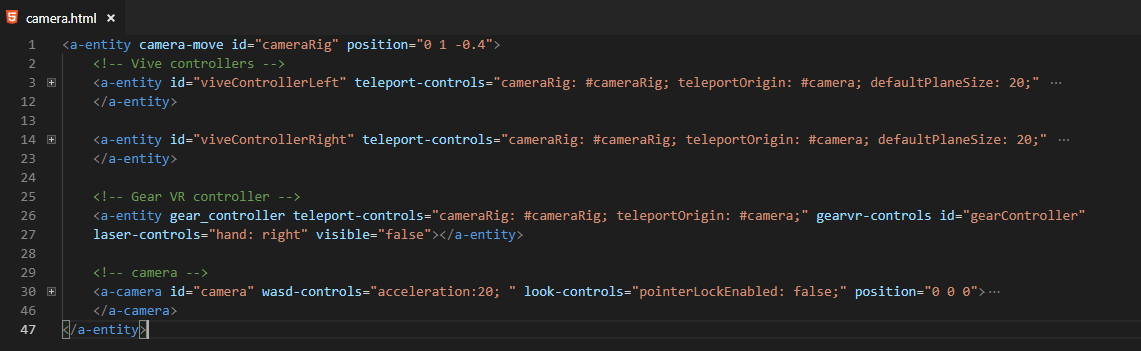
\includegraphics[width=\textwidth]{images/cameraHtml.png}
\begin{lstlisting}[language=HTML5, style=htmlcssjs]
<a-entity camera-move id="cameraRig" position="0 1 -0.4">
    <!-- Vive controllers -->
    <a-entity id="viveControllerLeft" teleport-controls="cameraRig: #cameraRig; teleportOrigin: #camera; defaultPlaneSize: 20;" 
    vive-controls="hand: left; model: false;" controller_6_d visible="false">
        <!-- some elements here ...  -->
    </a-entity>
    <a-entity id="viveControllerRight" teleport-controls="cameraRig: #cameraRig; teleportOrigin: #camera; defaultPlaneSize: 20;" 
    vive-controls="hand: right; model: false;" controller_6_d visible="false">
       <!-- some elements here ...  -->
    </a-entity>
    <!-- Gear VR controller -->
    <a-entity gear_controller teleport-controls="cameraRig: #cameraRig; teleportOrigin: #camera;" gearvr-controls id="gearController" 
    laser-controls="hand: right" visible="false"></a-entity>
    <!-- camera -->
    <a-camera id="camera" wasd-controls="acceleration:20; " look-controls="pointerLockEnabled: false;" position="0 0 0">
        <!-- some elements here ...  -->
    </a-camera>
</a-entity>
\end{lstlisting}
\label{fig:cameraHtml} 
\end{figure}
  
  Außer der manuellen Navigation wird auch die automatische Navigation implementiert. Das Event {\fontfamily{qcr}\selectfont raycaster-intersected} wird auf dasselbe Objekt emittiert, wenn das Objekt mit dem Zeiger überlappt. Dann bewegt sich die Kamera zu dem Objekt. Nach sechs Sekunden geht die Kamera wieder zurück. Wenn die Aktivitäten auf einem Objekt fertig sind, empfängt das Objekt kein Event mehr. (Abbildung ~\ref{fig:cameraMove})
  
\begin{figure}[ht]
\vspace*{1em}
\centering
\caption[Automatische Navigation]{Automatische Navigation}
%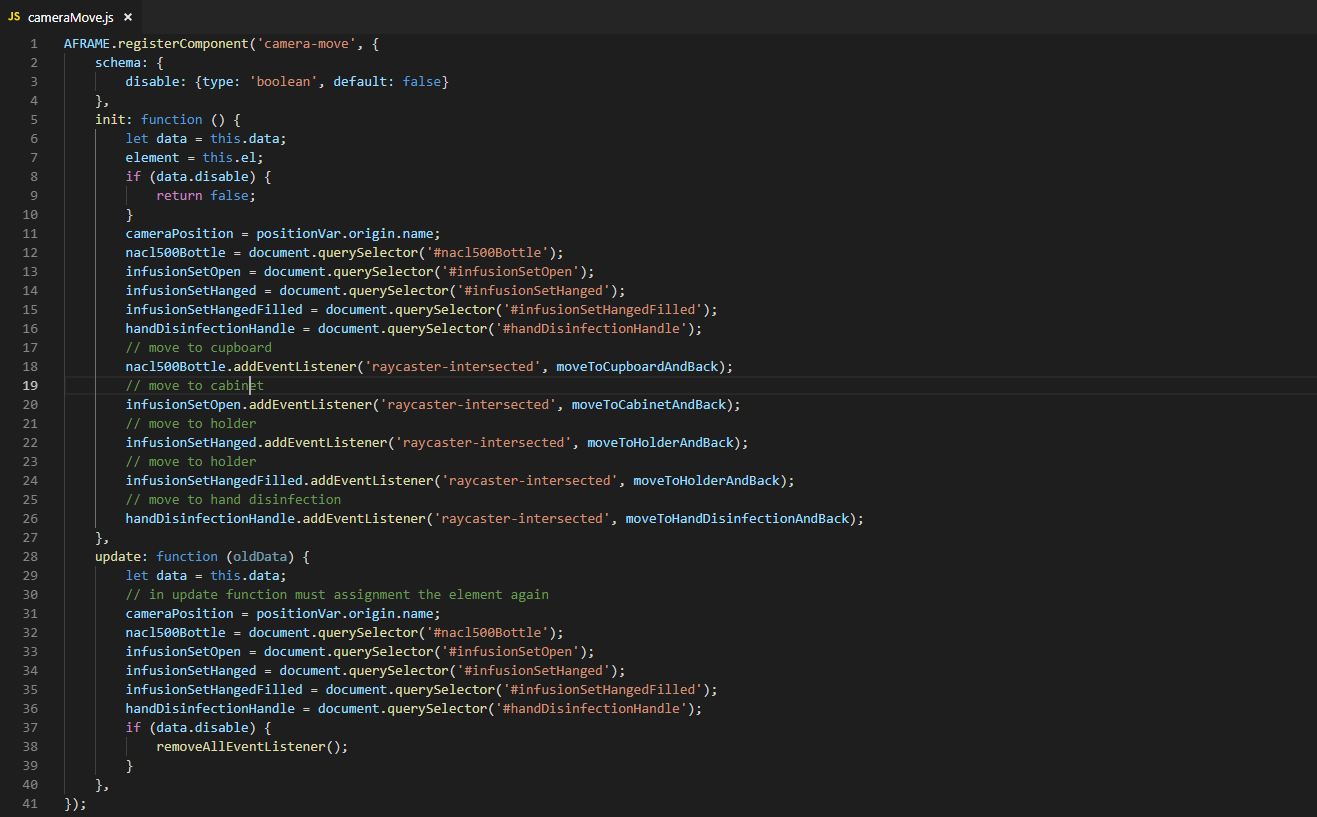
\includegraphics[width=\textwidth]{images/cameraMove.png}
\begin{lstlisting}[language=JavaScript, style=htmlcssjs]
AFRAME.registerComponent('camera-move', {
    schema: {
        disable: {type: 'boolean', default: false}
    },
    init: function () {
        let data = this.data;
        element = this.el;
        if (data.disable) {
            return false;
        }
        cameraPosition = positionVar.origin.name;
        // get more elements here ...
        handDisinfectionHandle = document.querySelector('#handDisinfectionHandle');
        nacl500Bottle.addEventListener('raycaster-intersected', moveToCupboardAndBack);
        infusionSetOpen.addEventListener('raycaster-intersected', moveToCabinetAndBack);
        infusionSetHanged.addEventListener('raycaster-intersected', moveToHolderAndBack);
        infusionSetHangedFilled.addEventListener('raycaster-intersected', moveToHolderAndBack);
        handDisinfectionHandle.addEventListener('raycaster-intersected', moveToHandDisinfectionAndBack);
    },
    update: function (oldData) {
        let data = this.data;
        // in update function must assign the elements again
        cameraPosition = positionVar.origin.name;
        // get more elements here ...
        handDisinfectionHandle = document.querySelector('#handDisinfectionHandle');
        if (data.disable) {
            removeAllEventListener();
        }
    },
});

\end{lstlisting}
\label{fig:cameraMove} 
\end{figure}
  
  \vspace{1em}
  \noindent
  \textbf{Manipulation}
  \vspace{1em}
  
  \noindent
  Die Manipulation auf PC und Smartphone wird mit dem built-in Component {\fontfamily{qcr}\selectfont a-cursor} implementiert (Abbildung ~\ref{fig:aCursorElement}). Um den Zeiger in der Mitte der Sicht darzustellen, wird {\fontfamily{qcr}\selectfont a-cursor} als ein Child-Component von {\fontfamily{qcr}\selectfont a-camera} eingesetzt.
  
 \begin{figure}[ht]
\vspace*{1em}
\centering
\caption[a-cursor Element]{a-cursor Element}
%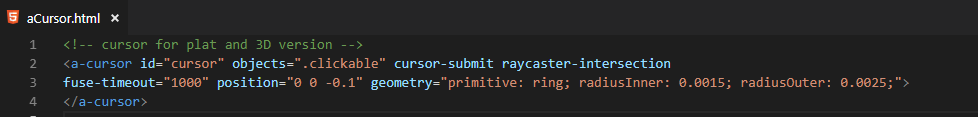
\includegraphics[width=\textwidth]{images/aCursorElement.png}
\begin{lstlisting}[language=HTML5, style=htmlcssjs]
<!-- cursor for plat and 3D version -->
<a-cursor id="cursor" objects=".clickable" cursor-submit raycaster-intersection 
fuse-timeout="1000" position="0 0 -0.1" geometry="primitive: ring; radiusInner: 0.0015; radiusOuter: 0.0025;">
</a-cursor>
\end{lstlisting}
\label{fig:aCursorElement} 
\end{figure}
  
  Das Attribut {\fontfamily{qcr}\selectfont objects} beschreibt, mit welchen Objekten man interagieren kann. Alle solche Objekte werden mit der HTML Klasse {\fontfamily{qcr}\selectfont clickable} bezeichnet. Mit dem Attribut {\fontfamily{qcr}\selectfont geometry} wird der Zeiger als ein Ring definiert.
  
  Als Standardeinstellung wird der Zeiger auf dem PC aktiviert, wenn die linke Taste von der Maus gedrückt wird. Mit dem Attribut {\fontfamily{qcr}\selectfont fuse-timeout} wird der Zeiger auf dem Smartphone konfiguriert. Die Wert 1000 bedeutet, dass der Zeiger aktiviert wird, wenn der Zeiger auf einem Objekt 1 Sekunde fokussiert.
  
  Das Attribut {\fontfamily{qcr}\selectfont raycaster-intersection} ist eine Entität der Klasse {\fontfamily{qcr}\selectfont raycaster-intersection}, welche die Funktion realisiert, dass der Zeiger farblich zu grün wechselt, wenn der Zeiger die Objekte trifft, mit denen interagiert werden kann.
  
  Das Event {\fontfamily{qcr}\selectfont raycaster-intersected} wird auf den Objekten selber emittiert, wenn das raycaster sich mit den Objekten überlappt. Im Gegenzug wird {\fontfamily{qcr}\selectfont raycaster-intersected-cleard} emittiert, wenn nichts mit dem Raycaster überlappt.
  
  Da {\fontfamily{qcr}\selectfont a-cursor} die Eigenschaften von Raycaster integriert hat, stehen die Events {\fontfamily{qcr}\selectfont raycaster-intersection} und {\fontfamily{qcr}\selectfont raycaster-intersection-cleard} für {\fontfamily{qcr}\selectfont a-cursor} zu Verfügung. (Abbildung ~\ref{fig:raycasterIntersection})
  
\begin{figure}[ht]
\vspace*{1em}
\centering
\caption[Raycaster Intersection]{Raycaster Intersection}
%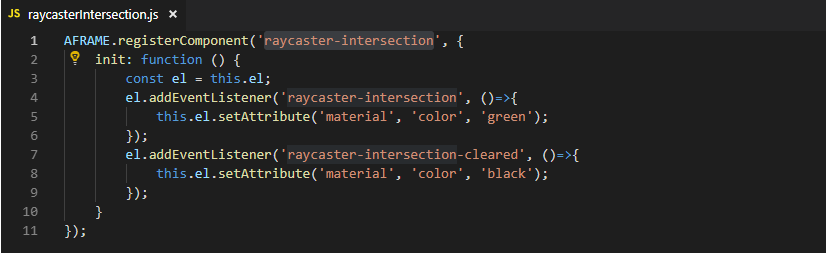
\includegraphics[width=\textwidth]{images/raycasterIntersection.png}
\begin{lstlisting}[language=JavaScript, style=htmlcssjs]
AFRAME.registerComponent('raycaster-intersection', {
    init: function () {
        const el = this.el;
        el.addEventListener('raycaster-intersection', ()=>{
            this.el.setAttribute('material', 'color', 'green');
        });
        el.addEventListener('raycaster-intersection-cleared', ()=>{
            this.el.setAttribute('material', 'color', 'black');
        });
    }
});
\end{lstlisting}
\label{fig:raycasterIntersection} 
\end{figure}
  
  Das Attribut {\fontfamily{qcr}\selectfont cursor-submit} ist zuständig für die Funktion, den Zeiger in rot darzustellen und ein entsprechendes Geräusch erklingen zu lassen, wenn der Zeiger aktiviert wird. (Abbildung ~\ref{fig:cursorSubmit})
  
\begin{figure}[ht]
\vspace*{1em}
\centering
\caption[Zeiger bestimmen]{Zeiger bestimmen}
%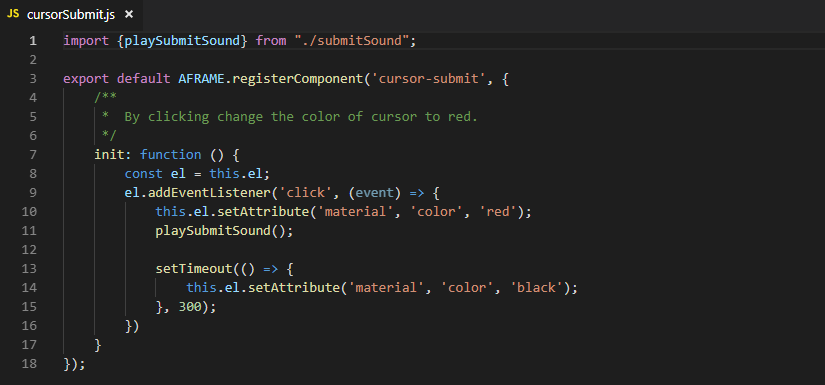
\includegraphics[width=\textwidth]{images/cursorSubmit.png}
\begin{lstlisting}[language=JavaScript, style=htmlcssjs]
import {playSubmitSound} from "./submitSound";
export default AFRAME.registerComponent('cursor-submit', {
    // By clicking change the color of cursor to red
    init: function () {
        const el = this.el;
        el.addEventListener('click', (event) => {
            this.el.setAttribute('material', 'color', 'red');
            playSubmitSound();
            setTimeout(() => {
                this.el.setAttribute('material', 'color', 'black');
            }, 300);
        })
    }
});
\end{lstlisting}
\label{fig:cursorSubmit} 
\end{figure}
  
  \subsubsection{Samsung Gear VR}
  Die Interaktionen für Samsung Gear VR sind abhängig von der Verfügbarkeit des Controllers.
  
  \vspace{1em}
  \noindent
  \textbf{Ohne Controller}
  \vspace{1em}
  
  \noindent
  Die Interaktionen von Samsung Gear VR ohne Controller sollen von den Funktionen für PC und Smartphone durch A-Frame automatisch angepasst werden. Allerdings taucht ein Problem bei der Anpassung an Gear VR auf: die Zeiger für jedes Auge überlappen sich nicht korrekt. Das heißt, dass zwei Zeiger in der Sicht erscheinen.
  
  Der Grund dafür ist, dass der Zeiger zu nahe an den Augen steht. Wenn der Zeiger weiter zu der Augen gelegt wird, ist der Zeiger eindeutig. Das führt jedoch zu der Situation, dass der Zeiger hinter manchen Objekten, wie der Krankenakte, ist. Wenn die Krankenakte auch weiter hinten eingesetzt wird, können die Informationen auf der Krankenakte nicht deutlich gesehen werden.
  
  Zwei mögliche Lösungen werden angegangen, Raycaster und große Skalierung.
  \begin{itemize}
      \item \textbf{Raycaster}: Die Idee des Raycasters ist, den Raycaster vom Controller zu den Augen zu bringen. Der Zeiger ist nicht mehr ein Ring, sondern eins aus dem Augen ausstrahlende Linie, sodass der Abstand zwischen Augen und Objekten keine Rolle spielt. Allerdings wird der Raycaster in Gear VR nicht richtig dargestellt. Die Linie wird in viele kurze Stückchen geschnitten. Und die Stückchen zeigen nicht in eine bestimmte Richtung. (Abbildung ~\ref{fig:GearVRRaycaster})
      
\begin{figure}[ht]
\vspace*{2.5em}
\centering
\caption[Raycaster in Gear VR]{Raycaster aus Kamera in Gear VR in A-Frame basic Scene}
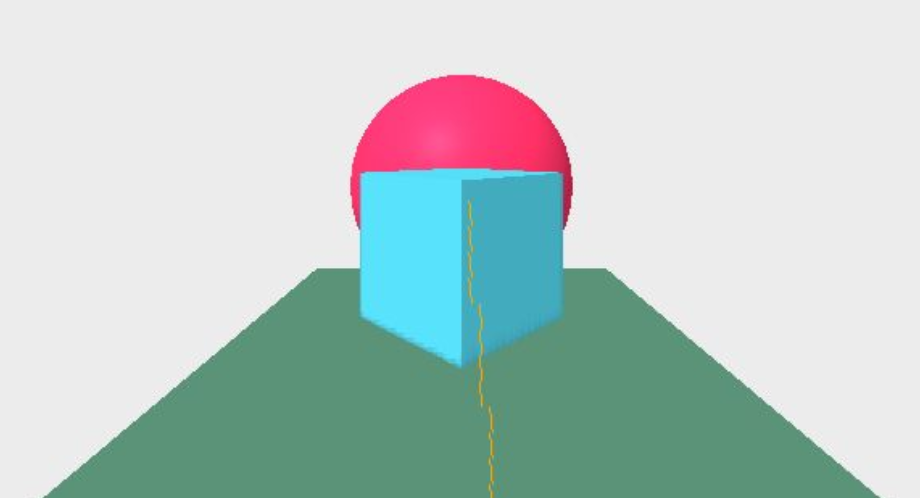
\includegraphics[width=\textwidth]{images/gearVRRaycaster.png}
\label{fig:GearVRRaycaster} 
\vspace*{1.5em}
\end{figure}
      
      \item \textbf{große Skalierung}: Der Zeiger und die anderen Objekte werden weit gelegt. Um die Objekte deutlicher zu sehen, werden alle Objekten vergrößert, sodass die relative Größe sich nicht verändert. Die Position der Kamera wird dafür angepasst.
      (Abbildung ~\ref{fig:GearVRCursor})
      
\begin{figure}[t]
\vspace*{1em}
\centering
\caption[vergrößerte Szene in Gear VR]{vergrößerte Szene in Gear VR}
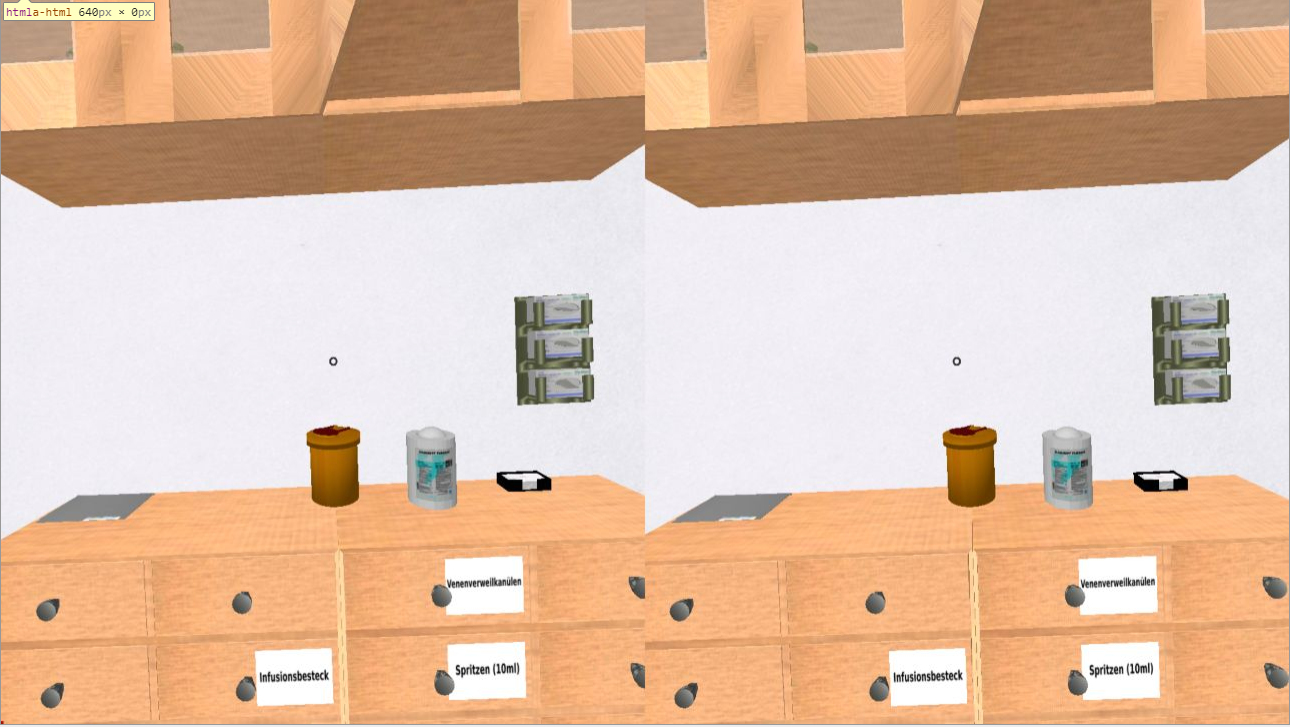
\includegraphics[width=\textwidth]{images/gearVRCursor.png}
\label{fig:GearVRCursor} 
\end{figure}
      
  \end{itemize}
  
  Obwohl die zweite Möglichkeit keine optimale Lösung ist, weil der Nutzer sich fühlt, dass er selber ein Riese ist, ist es besser als geschnittenes Raycaster, deswegen wird diese Lösung eingesetzt. 
  
  \vspace{1em}
  \noindent
  \textbf{Mit Controller}
  \vspace{1em}
  
  \noindent
  Navigation und Manipulation werden durch den Controller aktiviert.
  
  Das Element von Gear VR Controller wird mit dem Element der Kamera zusammen in dem Element mit ID {\fontfamily{qcr}\selectfont cameraRig} eingepackt. Die Bewegung der Kamera wird durch die Translation von {\fontfamily{qcr}\selectfont cameraRig} ermöglicht, sodass die relative Position zwischen der Kamera und dem Controller während der Bewegung behalten wird.
  
  Mit dem built-in Component {\fontfamily{qcr}\selectfont teleport-controls} wird die Navigation implementiert. Das Attribut{\fontfamily{qcr}\selectfont cameraRig} beschreibt das Element, das sich zu der bezeichneten Position bewegt. Das Attribut {\fontfamily{qcr}\selectfont teleportOrigin} beschreibt das Element, das als der Ursprung des Elements {\fontfamily{qcr}\selectfont cameraRig} gilt.
  
  Wenn das Trackpad auf dem Gear VR Controller gedrückt wird, wird die Position festgelegt. Solange der Trackpad losgelöst wird, bewegt sich das Element {\fontfamily{qcr}\selectfont cameraRig} zu der festgelegten Position. Die Position der Kamera auf den X und Z Achsen sind die gleichen wie die festgelegten Positionen.
  
  Die Manipulation wird durch das Component {\fontfamily{qcr}\selectfont laser-controls} realisiert. Mit dem Component wird nicht nur der Gear VR Controller, sondern auch Daydrame Controller usw. (Abbildung ~\ref{fig:GearVRControllerElement} \& Abbildung ~\ref{fig:GearVRWithController})
  
\begin{figure}[ht]
\vspace*{1em}
\centering
\caption[Gear VR Controller Element]{Gear VR Controller Element}
%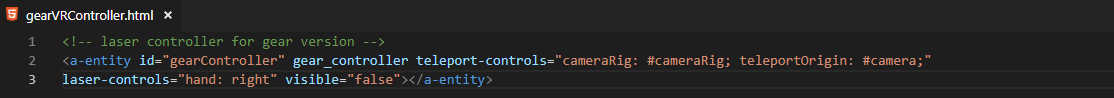
\includegraphics[width=\textwidth]{images/gearVRControllerElement.png}
\begin{lstlisting}[language=HTML5, style=htmlcssjs]
<!-- laser controller for gear version -->
<a-entity id="gearController" gear_controller teleport-controls="cameraRig: #cameraRig; teleportOrigin: #camera;" laser-controls="hand: right" visible="false"></a-entity>
\end{lstlisting}
\label{fig:GearVRControllerElement} 
\end{figure}
  
\begin{figure}[ht]
\vspace*{1em}
\centering
\caption[Gear VR mit Controller]{Gear VR mit Controller}
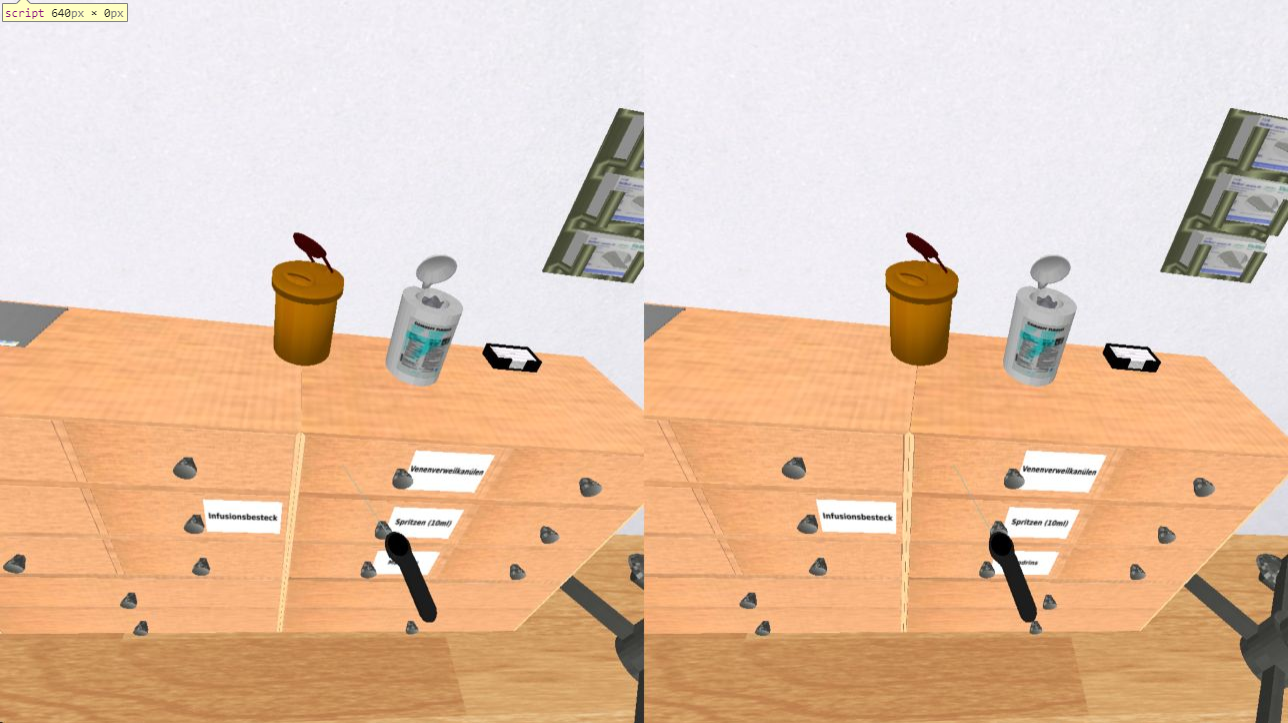
\includegraphics[width=\textwidth]{images/gearVRWithController.png}
\label{fig:GearVRWithController} 
\end{figure}
  
  \subsubsection{HTC Vive}
  
  Die Navigation von HTC Vive wird durch das Component {\fontfamily{qcr}\selectfont teleport-controls} ist so implementiert wie bei der Gear VR.
  
  \vspace{1em}
  \noindent
  \textbf{Component vive-controls}
  \vspace{1em}
  
  \noindent
  Durch das built-in Component {\fontfamily{qcr}\selectfont vive-controls} werden die Vive Controllers anerkannt. Mit dem Attribut {\fontfamily{qcr}\selectfont model} wird die Darstellung des Modells von Controller konfiguriert. Da die Controllers als Hände gezeigt werden, wird das Attribut als {\fontfamily{qcr}\selectfont false} eingerichtet. (Abbildung ~\ref{fig:viveControllerElement})
  
\begin{figure}[ht]
\vspace*{1em}
\centering
\caption[Vive Controller Element]{Vive Controller Element}
%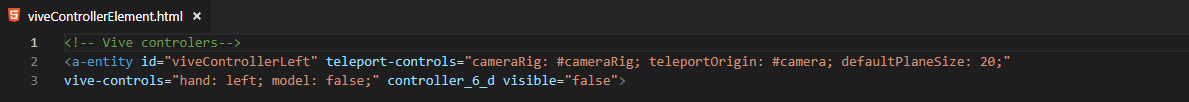
\includegraphics[width=\textwidth]{images/viveControllerElement.png}
\begin{lstlisting}[language=HTML5, style=htmlcssjs]
<!-- Vive controlers-->
<a-entity id="viveControllerLeft" teleport-controls="cameraRig: #cameraRig; teleportOrigin: #camera; defaultPlaneSize: 20;" vive-controls="hand: left; model: false;" controller_6_d visible="false"></a-entity>
\end{lstlisting}
\label{fig:viveControllerElement} 
\end{figure}
  
  Nach der Erkennung der Controllers werden Events {\fontfamily{qcr}\selectfont triggerdown} und {\fontfamily{qcr}\selectfont triggerup} ausgelöst, wenn der Hair-Trigger gedrückt und losgelöst wird. Um die Nachrichten über die Aktivität des Controllers auszubreiten, wird Observer Pattern verwendet.
  
  Die Controller relevanten Funktionen bei unterschiedlichen Objekten melden sich bei den \glqq Observerables\grqq\ für {\fontfamily{qcr}\selectfont triggerdown} und {\fontfamily{qcr}\selectfont triggerup}. Wenn der Hair-Trigger gedrückt oder losgelöst wird, wird die Information (Name von Event, ID von Controller, globale Position von Controller) an alle \glqq Observers\grqq\ geschickt. (Abbildung ~\ref{fig:controller6D})
  
\begin{figure}[ht]
\vspace*{1em}
\centering
\caption[6 DoF Controller]{6 DoF Controller}
%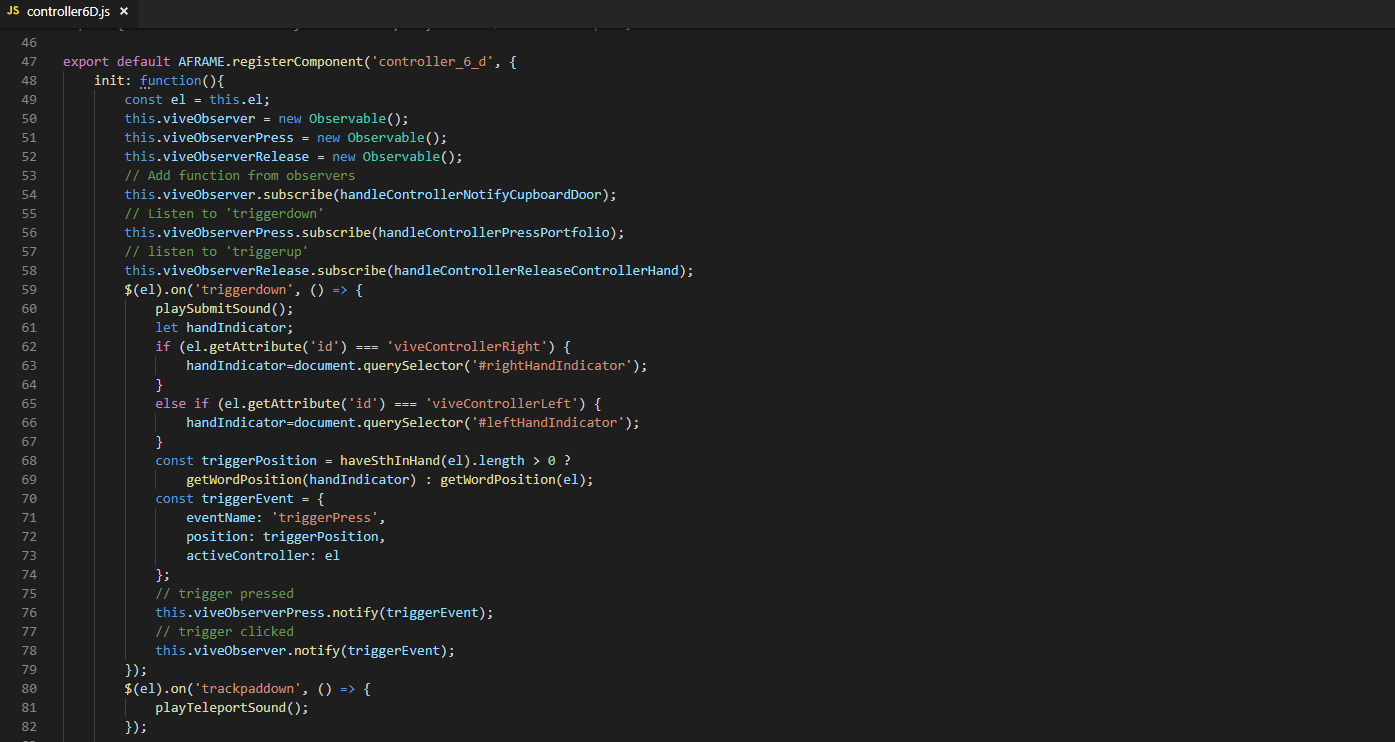
\includegraphics[width=\textwidth]{images/controller6D.png}
\begin{lstlisting}[language=JavaScript, style=htmlcssjs]
export default AFRAME.registerComponent('controller_6_d', {
    init: function(){
        const el = this.el;
        this.viveObserver = new Observable();
        this.viveObserverPress = new Observable();
        this.viveObserverRelease = new Observable();
        // Add function from observers
        this.viveObserver.subscribe(handleControllerNotifyCupboardDoor);
        // Listen to 'triggerdown'
        this.viveObserverPress.subscribe(handleControllerPressPortfolio);
        // listen to 'triggerup'
        this.viveObserverRelease.subscribe(handleControllerReleaseControllerHand);
        $(el).on('triggerdown', () => {
            playSubmitSound();
            let handIndicator;
            if (el.getAttribute('id') === 'viveControllerRight') {
                handIndicator=document.querySelector('#rightHandIndicator');
            }
            else if (el.getAttribute('id') === 'viveControllerLeft') {
                handIndicator=document.querySelector('#leftHandIndicator');
            }
            const triggerPosition = haveSthInHand(el).length > 0 ?
                getWorldPosition(handIndicator) : getWorldPosition(el);
            const triggerEvent = {
                eventName: 'triggerPress',
                position: triggerPosition,
                activeController: el
            };
            // trigger pressed
            this.viveObserverPress.notify(triggerEvent);
            // trigger clicked
            this.viveObserver.notify(triggerEvent);
        });
        $(el).on('trackpaddown', () => {
            playTeleportSound();
        });
        // handle event triggerup and trackpadup here ...
\end{lstlisting}
\label{fig:controller6D} 
\end{figure}
  
  Um die globale Position zu errechnen, wird die Funktion von three.js verwendet. Die A-Frame Objekte sind eigentlich verpackte three.js Objekte, deswegen ist die Verwendung von three.js in A-Frame barrierefrei. Das gilt als ein Vorteil von A-Frame. (Abbildung ~\ref{fig:getWorldPosition})
  
\begin{figure}[ht]
\vspace*{1em}
\centering
\caption[get global position]{get global position}
%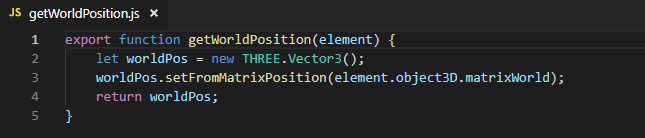
\includegraphics[width=\textwidth]{images/getWorldPosition.png}
\begin{lstlisting}[language=JavaScript, style=htmlcssjs]
export function getWorldPosition(element) {
    let worldPos = new THREE.Vector3();
    worldPos.setFromMatrixPosition(element.object3D.matrixWorld);
    return worldPos;
}
\end{lstlisting}
\label{fig:getWorldPosition} 
\end{figure}
  
  \vspace{1em}
  \noindent
  \textbf{Prüfung mit Raycaster}
  \vspace{1em}
  
  \noindent
  Ein aus den Augen ausstrahlender versteckter Raycaster wird in dem Element {\fontfamily{qcr}\selectfont a-camera} eingesetzt. Wenn die Krankenakte, Infusionsflasche und Infusionsbesteck überprüft werden sollen, wird der Raycaster gezeigt, um die Überprüfung durchzuführen. Wenn der Raycaster die richtige Position trifft, wird das Event {\fontfamily{qcr}\selectfont raycaster-intersection} ausgelöst, und der Raycaster wird in grün dargestellt, ansonsten in orange. Wenn die Überprüfung fertig ist, die relevanten Zustände für die Prüfungen als {\fontfamily{qcr}\selectfont true} gesetzt sind, wird der Raycaster wieder versteckt.
  
  \vspace{1em}
  \noindent
  \textbf{Zustände für Vive Controller}
  \vspace{1em}
  
  \noindent
  Weil die Manipulation mit Vive Controllern große Freiheiten hat, und nicht jede Ausführung einer Aktivität den Fortschritt fördert, wird eine neue Liste für die Zustände der Vive Controller und die entsprechenden Funktionen erstellt.
  
  Zum Beispiel wird der Wert des Zustands für Vive Controller {\fontfamily{qcr}\selectfont portfolioInHand} als die ID des Controllers, der mit der Krankenakte interagiert, gespeichert, und die Zustände an die Observers (Krankenakte usw.) geschickt. Solange die Änderung des Zustands im Component der Krankenakte übergeben wird, wird das Element der Krankenakte in dem Element des entsprechenden Controllers eingezogen. (Abbildung ~\ref{fig:controller6D} \& Abbildung ~\ref{fig:portfolioPress})
  
\begin{figure}[ht]
\vspace*{1em}
\centering
\caption[Bearbeitung der Krankenakte]{Bearbeitung der Krankenakte}
%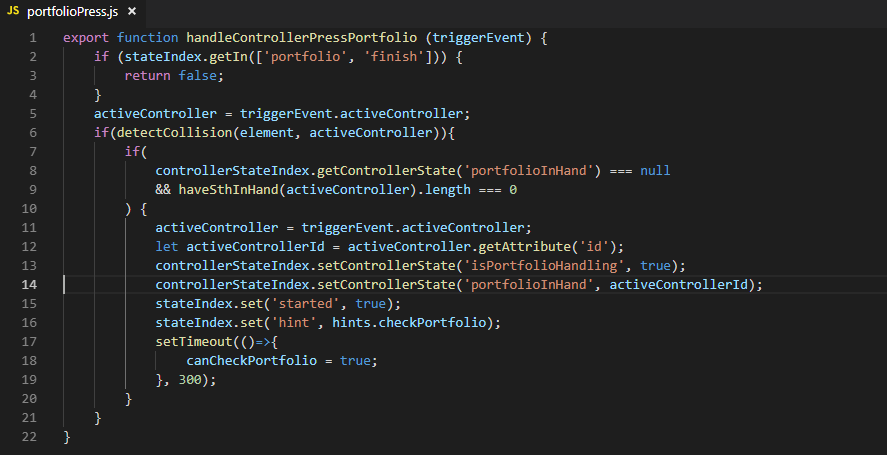
\includegraphics[width=\textwidth]{images/portfolioPress.png}
\begin{lstlisting}[language=JavaScript, style=htmlcssjs]
export function handleControllerPressPortfolio (triggerEvent) {
    if (stateIndex.getIn(['portfolio', 'finish'])) {
        return false;
    }
    activeController = triggerEvent.activeController;
    if(detectCollision(element, activeController)){
        if(
            controllerStateIndex.getControllerState('portfolioInHand') === null
            && haveSthInHand(activeController).length === 0
        ) {
            activeController = triggerEvent.activeController;
            let activeControllerId = activeController.getAttribute('id');
            controllerStateIndex.setControllerState('isPortfolioHandling', true);
            controllerStateIndex.setControllerState('portfolioInHand', activeControllerId);
            stateIndex.set('started', true);
            stateIndex.set('hint', hints.checkPortfolio);
            setTimeout(()=>{
                canCheckPortfolio = true;
            }, 300);
        }
    }
}
\end{lstlisting}
\label{fig:portfolioPress} 
\end{figure}
  
  \vspace{1em}
  \noindent
  \textbf{Attribute Veränderung}
  \vspace{1em}
  
  \noindent
  Wenn ein Element in dem Controller Element eingezogen oder aus dem Controller ausgezogen wird, wird die Dimension der Koordinaten geändert. Deshalb muss das Attribut Position neu berechnet und umgesetzt werden.
  
  Normalerweise kann das Attribut direkt mit dem Befehl {\fontfamily{qcr}\selectfont setAttribute} konfiguriert werden. Allerdings sind die 3D A-Frame Objekte viel größer als 2D Objekte, sodass die DOM Manipulation länger dauert. Deshalb passiert es, dass die Änderung des Attributs vor dem Umzug des DOM Elements geschafft wird. Und nach dem Umzug wird das Attribut wieder zurückgesetzt.
  
  Um das Problem zu lösen, muss die DOM Funktion {\fontfamily{qcr}\selectfont MutationObserver} verwendet werden. Die Funktion {\fontfamily{qcr}\selectfont MutationObserver} ist zuständig dafür, die Änderung der gegebenen Attribute eines Elements zu beobachten. Wenn die Änderung fertig ist, wird eine Nachricht an alle Observers geschickt.
  
  Weil die DOM Manipulation sehr häufig ist und fast alle aufwendigen Änderungen mit den Controllern zu tun haben, wird die Funktion {\fontfamily{qcr}\selectfont MutationObserver} in einer Klasse {\fontfamily{qcr}\selectfont controllerActions} verpackt, um die Verwendung zu vereinfachen.
  
  Die {\fontfamily{qcr}\selectfont MutationObserver} beachten die {\fontfamily{qcr}\selectfont childList} des eingegebenen Controllers. Wenn die Einfügung und Entfernung der Child Elements des Controllers fertig ist, werden die eingegebenen Attribute eingesetzt. (Abbildung ~\ref{fig:controllerAction})
  
\begin{figure}[ht]
\vspace*{1em}
\centering
\caption[Veränderung der Attribute]{Veränderung der Attribute}
%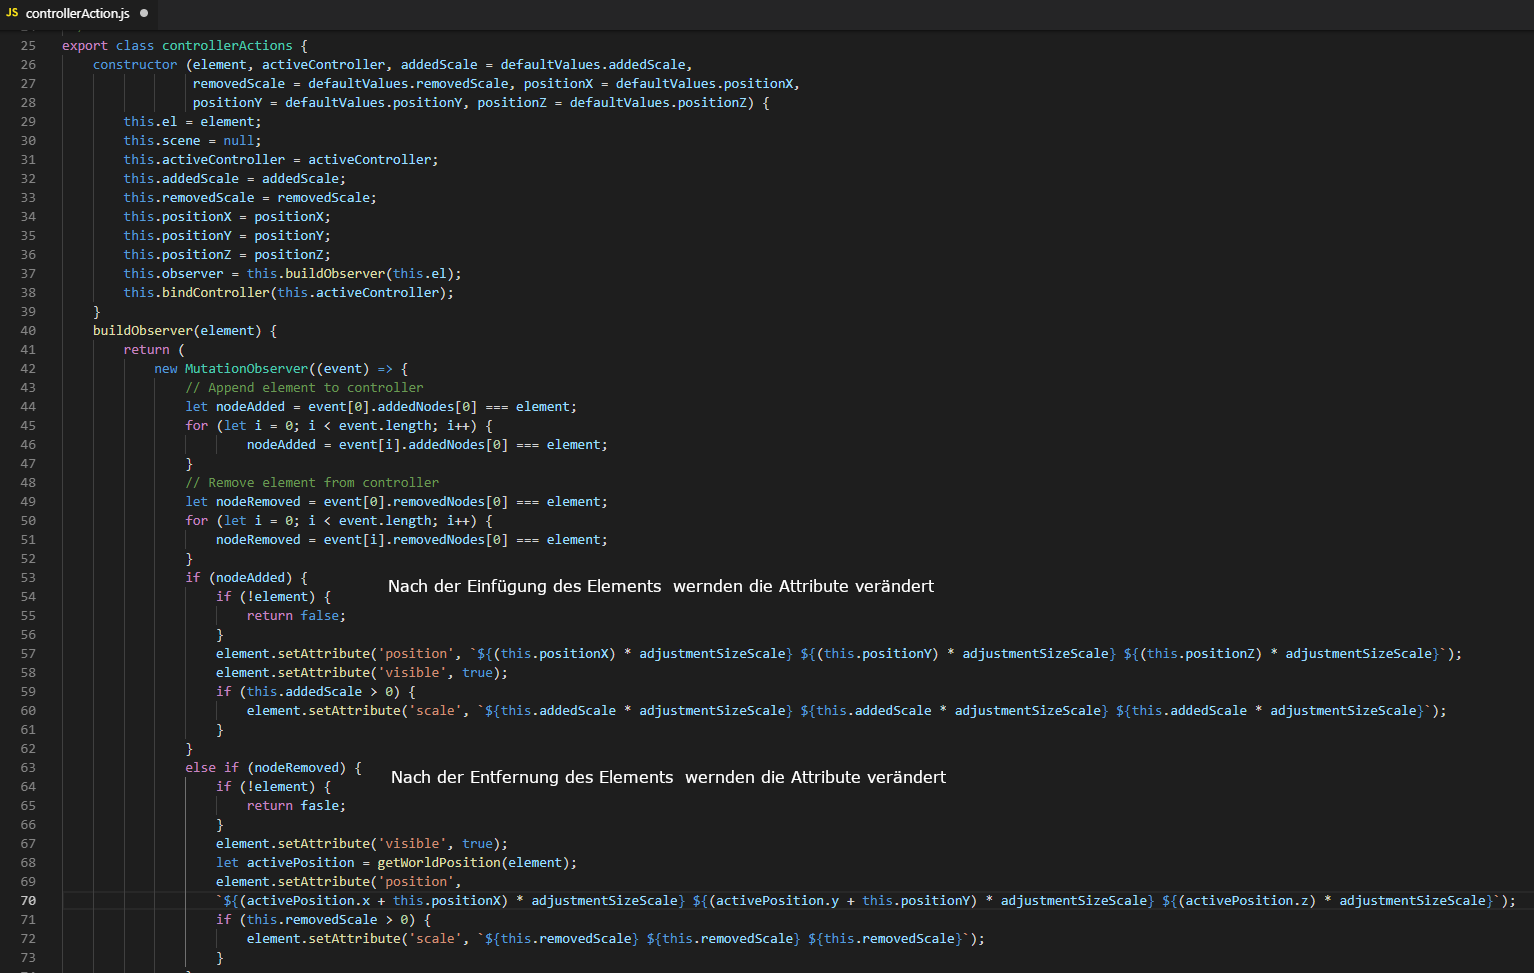
\includegraphics[width=\textwidth]{images/controllerAction.png}
\begin{lstlisting}[language=JavaScript, style=htmlcssjs]
export class controllerActions {
    constructor (element, activeController, 
        // pass the value of attribute to change here ...
    ) {
        this.el = element;
        this.scene = null;
        this.activeController = activeController;
        // get values from parameters here ...
        this.observer = this.buildObserver(this.el);
        this.bindController(this.activeController);
    }
    buildObserver(element) {
        return (
            new MutationObserver((event) => {
                // append element to controller
                let nodeAdded = event[0].addedNodes[0] === element;
                for (let i = 0; i < event.length; i++) {
                        nodeAdded = event[i].addedNodes[0] === element;
                }
                // remove element from controller
                let nodeRemoved = event[0].removedNodes[0] === element;
                for (let i = 0; i < event.length; i++) {
                    nodeRemoved = event[i].removedNodes[0] === element;
                }
                if (nodeAdded) {
                    if (!element) {
                        return false;
                    }
                    // change attribute after adding to controller here ...
                }
                else if (nodeRemoved) {
                    if (!element) {
                        return fasle;
                    }
                    // change attribute after removing from controller here ...
                }
            })
        );
    }
\end{lstlisting}
\label{fig:controllerAction} 
\end{figure}
  
  \vspace{1em}
  \noindent
  \textbf{Hinweis-Box}
  \vspace{1em}
  
  \noindent
  Die Hinweis-Box wird durch das built-in Element {\fontfamily{qcr}\selectfont a-box} implementiert. Durch die Konfiguration des Attributs {\fontfamily{qcr}\selectfont material} wird die Hinweis-Box in halb-transparentem rot dargestellt, wenn ein Objekt, beispielsweise die Krankenakte, in der Hand ist. Die Hinweis-Box beobachtet die Zustände aller Objekte. Wenn alle nötige Aktivitäten für das Objekt fertig gemacht sind, z.B. Überprüfung der Krankenakte, werden die Änderungen der entsprechenden Zustände von der Hinweis-Box erkannt. Nach der Erkennung wird das Attribut {\fontfamily{qcr}\selectfont material} in grün umgeschrieben.
  
  Wenn die Kollision zwischen der grünen Hinweis-Box und dem Objekt in der Hand während des Loslösens auf den Hair-Trigger des Controllers detektiert wird, wird der entsprechende Zustand geändert und das Objekt auf den entsprechend Platz gelegt.
  
  image: M5 toggleBoxPortfolio .........
  
  \vspace{1em}
  \noindent
  \textbf{Kollisionserkennung}
  \vspace{1em}
  
  \noindent
  Die Funktion Kollisionserkennung wird durch die Funktionen von three.js implementiert. Die zwei Objekte werden erst durch die Funktion {\fontfamily{qcr}\selectfont setFromObject} als Würfel umgerechnet. Durch die Funktion {\fontfamily{qcr}\selectfont intersectsBox} wird es überprüft, ob zwei Würfel überlappt sind, damit die Kollision zu erkennen.
  
  Allerdings ist die Methode keine optimale Lösung. Wenn der Rahmen des Objektes kein Würfel ist, ist die Kollisionserkennung ungenau. (Abbildung ~\ref{fig:collisionDetection})
  
\begin{figure}[ht]
\vspace*{1em}
\centering
\caption[Kollisionserkennung]{Kollisionserkennung}
%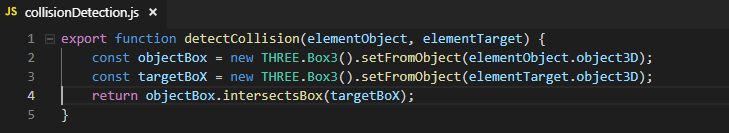
\includegraphics[width=\textwidth]{images/collisionDetection.png}
\begin{lstlisting}[language=JavaScript, style=htmlcssjs]
export function detectCollision(elementObject, elementTarget) {
    const objectBox = new THREE.Box3().setFromObject(elementObject.object3D);
    const targetBoX = new THREE.Box3().setFromObject(elementTarget.object3D);
    return objectBox.intersectsBox(targetBoX);
}
\end{lstlisting}
\label{fig:collisionDetection} 
\end{figure}
  
  \vspace{1em}
  \noindent
  \textbf{Freier Fall}
  \vspace{1em}
  
  \noindent
  Die Objekte können aus den Händen fallen, wenn der Hair-Trigger losgelöst wird.
  
  Das Fallen wird so simuliert, dass in jedem bestimmten Zeitraum (z.B. 0.01 Millisekunde) die Position auf der Y-Achse des Objektes eine Geschwindigkeit reduziert wird. Laut der Formel der Geschwindigkeit des freien Falls 
  
  image: Formel Geschwindigkeit V(t) = gt, g = 9.8 .........
  
  kann die Geschwindigkeit so errechnet {\fontfamily{qcr}\selectfont speed = speed + accelerate} werden. 
  %TODO 9.8 ist die Erdbeschleunigung und wird in m/s^2 eig angegeben
  %TODO: nicht ganz klar (von Le)
  Da das reale Erdbeschleunigung ist 9.8 m/s, soll die konstante Wert {\fontfamily{qcr}\selectfont accelerate} 0.098 sein. Aber in der simulierten VR Umgebung fällt das Objekt zu schnell, sodass das Fallen nicht deutlich gemerkt werden kann. Um bessere Benutzererfahrung zu implementieren, wird die Wert {\fontfamily{qcr}\selectfont accelerate} als 0.049 befestigt.
  
  Um den passende Zeitpunkt zu finden, das Fallen zu beenden, wird jede 0.01 Millisekunde die Kollision auf Y-Achse detektiert. Allerdings könnte es passieren, dass vor der Detektion das Objekt in der letzten 0.01 Millisekunde schon in anderem Objekt, beispielsweise in den Boden, gefallen ist. Wenn das Objekt sehr dünn ist, z.B. Namenetikett, wird es nicht mehr gesehen.
  
  Um das Problem zu vermeiden, wird eine Variable {\fontfamily{qcr}\selectfont lowestY} benutzt. Damit kann eine neue Ebene erstellt werden, die als eine Kollisions-Ebene auf der Y-Achse gilt. Mit der Hilfe der neuen Ebene, kann das Fallen des Objektes früher beendet werden. Allerdings kann es passieren, dass das Objekt oberhalb des Boden liegt.
  
  Außer Boden (Y = 0) können andere Objekte eine wichtige Rolle bei dem Fallen spielen, z.B die Arbeisoberfläche auf den Schubladentisch. Um den Bereich der Arbeitsoberfläche zu finden, muss die Koordination des Rahmen des Schubladentisches in der Szene gefunden werden. Das A-Frame Objekt wird erst zum three.js Box3 Objekt umgesetzt. Der Wert der Position des Rahmens des Objektes kann aus der Eigenschaft {\fontfamily{qcr}\selectfont boundingBox} gefunden werden. Die höchste Fläche gilt als der Kollisionsbereich. (Abbildung ~\ref{fig:fallDown})
  
\begin{figure}[ht]
\vspace*{1em}
\centering
\caption[Freier Fall]{Freier Fall}
%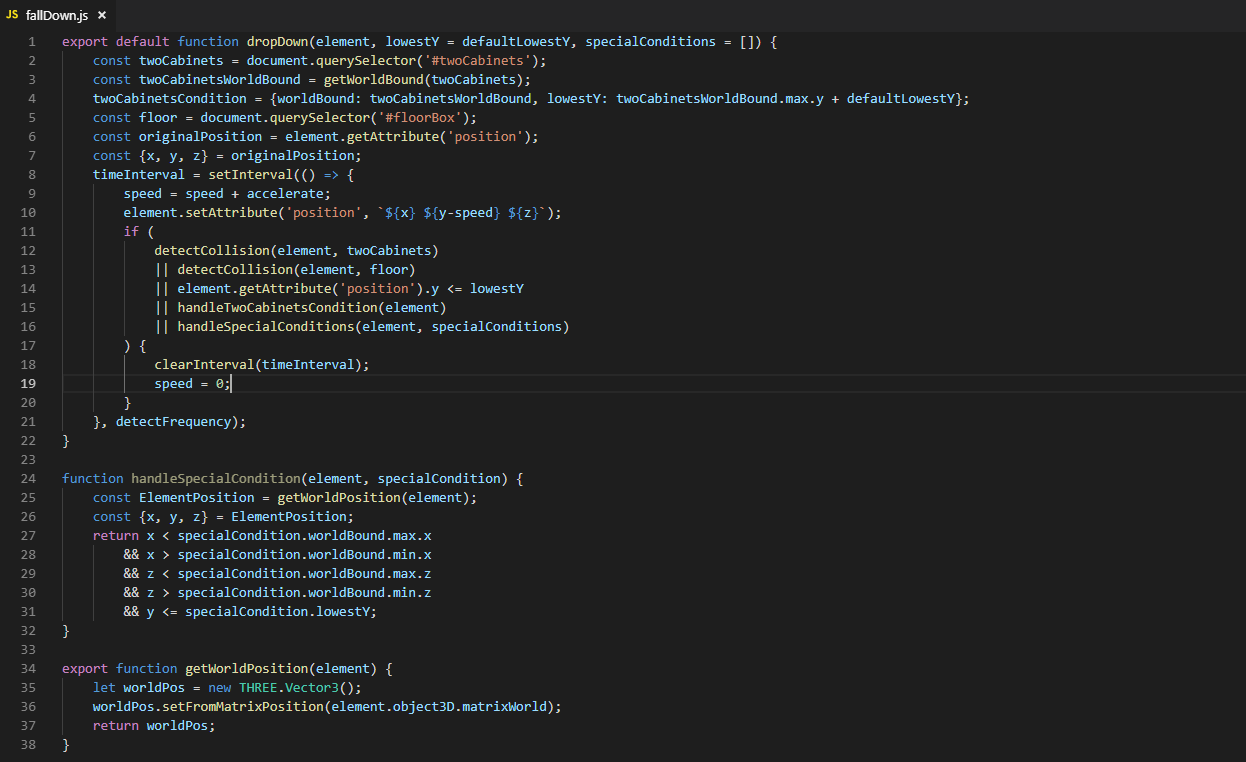
\includegraphics[width=\textwidth]{images/fallDown.png}
\begin{lstlisting}[language=JavaScript, style=htmlcssjs]
export default function dropDown(element, lowestY = defaultLowestY, specialConditions = []) {
    const twoCabinets = document.querySelector('#twoCabinets');
    const twoCabinetsWorldBound = getWorldBound(twoCabinets);
    twoCabinetsCondition = {worldBound: twoCabinetsWorldBound, lowestY: twoCabinetsWorldBound.max.y + defaultLowestY};
    const floor = document.querySelector('#floorBox');
    const originalPosition = element.getAttribute('position');
    const {x, y, z} = originalPosition;
    timeInterval = setInterval(() => {
        speed = speed + accelerate;
        element.setAttribute('position', `${x} ${y-speed} ${z}`);
        if (
            detectCollision(element, twoCabinets)
            || detectCollision(element, floor)
            || element.getAttribute('position').y <= lowestY
            || handleTwoCabinetsCondition(element)
            || handleSpecialConditions(element, specialConditions)
        ) {
            clearInterval(timeInterval);
            speed = 0;
        }
    }, detectFrequency);
}
export function getWorldBound(element) {
    let boundingBox = new THREE.Box3().setFromObject(element.object3D);
}
\end{lstlisting}
\label{fig:fallDown} 
\end{figure}
  
  \subsubsection{Möglichkeit der Verbesserung}
  Die kürzere Ladezeit der Applikation führt zur besseren Benutzererfahrung. Die Größe der Dateien spielt eine wichtige Rolle bei der Ladung.
  
  Nicht alle Geräte können sich mit der HTC Vive verbinden, deswegen wäre es besser, dass die Codes, die mit HTC Vive zu tun haben, in eone eigene Datei geschrieben und in einem Verzeichnis gespeichert werden. Dieses Verzeichnis wird geladen, nur wenn die HTC Vive Controller erkannt werden.
  
  So wird die Ladezeit für die Geräte, außer der HTC Vive, verringert.
  
 \subsection{Geräte anpassen}
 Anpassende Interaktionen werden für unterschiedliche Geräte gestaltet und implementiert. Um die Szene lebhafter darzustellen, die Interaktion barrierefrei durchzuführen und die falsche Initialisierung der Position der Kamera (Bug von A-Frame) zu beheben, muss die Applikation für die unterschiedlichen Geräte während des Ladens konfiguriert werden.
 
 Durch die Funktion {\fontfamily{qcr}\selectfont navigator.userAgent} wird die Informationen über den Browser ausgelesen. Dadurch werden die Typen der Geräten (PC, Smartphone, GearVR) unterschieden. Durch das Event {\fontfamily{qcr}\selectfont gamepadconnected} wird der verbundene Controller (GearVR Controller, Vive Controller) erkannt. Damit wird die Mode auf dem PC (flach, VR) und Gear VR (ohne Controller, mit Controller) unterschieden. Durch das Event {\fontfamily{qcr}\selectfont enter-vr} wird die Mode auf Smartphone (flach, Cardboard) unterschieden. (Abbildung ~\ref{fig:geraeteAnpassen} \& Tabelle ~\ref{tab:geraeteAnpassen}) 
 
\begin{figure}[ht]
\vspace*{1em}
\centering
\caption[Geräte erkennen]{Geräte erkennen}
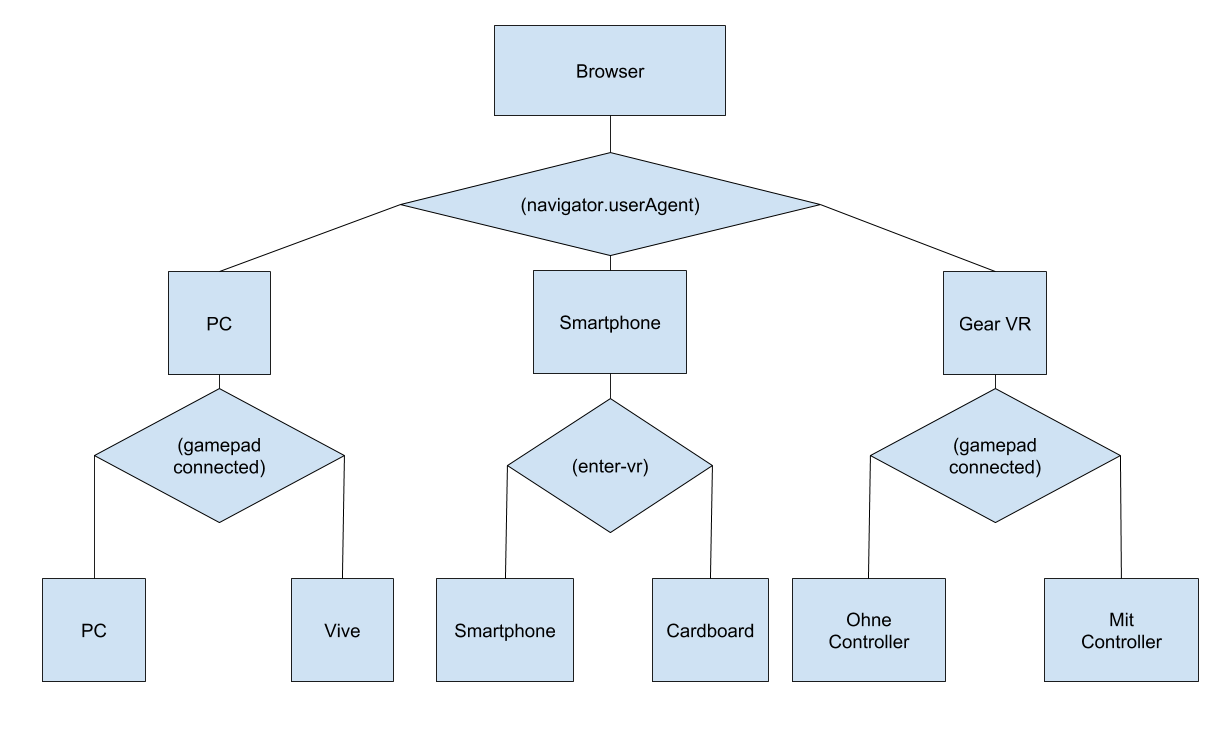
\includegraphics[width=\textwidth]{images/geraeteAnpassen.png}
\label{fig:geraeteAnpassen} 
\end{figure}

\begin{table}
\centering
\caption{Anpassung der Geräten}
\label{tab:geraeteAnpassen}
\begin{tabular}{|l|l|l|l|l|l|} 
\toprule
PC & Vive                                                                           & \begin{tabular}[c]{@{}l@{}}Smart-\\phone\end{tabular} & Cardboard                                                            & \begin{tabular}[c]{@{}l@{}}Gear VR Ohne\\Controller\end{tabular}     & \begin{tabular}[c]{@{}l@{}}Gear VR Mit\\Controller\end{tabular}                 \\ 
\hline
   & \begin{tabular}[c]{@{}l@{}}Ring Zeiger\\entfernen\end{tabular}                 &                                                       & \begin{tabular}[c]{@{}l@{}}Kamera\\Position\\einstellen\end{tabular} & \begin{tabular}[c]{@{}l@{}}Objekte\\skalieren\end{tabular}           & \begin{tabular}[c]{@{}l@{}}Ring Zeiger\\entfernen\end{tabular}                  \\ 
\cline{2-2}\cline{4-6}
   & \begin{tabular}[c]{@{}l@{}}Objekte\\skalieren\end{tabular}                     &                                                       &                                                                      & \begin{tabular}[c]{@{}l@{}}Kamera\\Position\\einstellen\end{tabular} & \begin{tabular}[c]{@{}l@{}}Automatische\\Navigation\\deaktivieren\end{tabular}  \\ 
\cline{2-2}\cline{5-6}
   & \begin{tabular}[c]{@{}l@{}}Kamera\\Position\\einstellen\end{tabular}           &                                                       &                                                                      &                                                                      & \begin{tabular}[c]{@{}l@{}}Objekte\\skalieren\end{tabular}                      \\ 
\cline{2-2}\cline{6-6}
   & \begin{tabular}[c]{@{}l@{}}Automatische\\Navigation\\deaktivieren\end{tabular} &                                                       &                                                                      &                                                                      & \begin{tabular}[c]{@{}l@{}}Gear VR\\Controller\\darstellen\end{tabular}         \\ 
\cline{2-2}\cline{6-6}
   & \begin{tabular}[c]{@{}l@{}}Vive\\Controller\\darstellen\end{tabular}           &                                                       &                                                                      &                                                                      &                                                                                 \\
\bottomrule
\end{tabular}
\end{table}
 
 \subsection{Töne}
 Die Töne sind wichtig, um eine lebhaftere Simulation aufzubauen. Alle realen Geräusche werden während der Übung im realen Skillslab der Fachhochschule Bielelfeld aufgenommen. Die Größe ist ca. 14 MB. Es ist zu groß, um es in einer webbasierten Applikation einzufügen, weil es zu langer Zeit für das Laden führt. Deswegen werden nur die Geräusche für die Feedbacks von Controllern eingesetzt.
 
 Vier Geräusche werden bei der Kamera eingesetzt, und für den Druck und die Loslösung des Hair-Triggers und dem Trackpad angepasst. Die built-in Funktion {\fontfamily{qcr}\selectfont playSound} wird in dem Objekt {\fontfamily{qcr}\selectfont sound} von {\fontfamily{qcr}\selectfont components} eingepackt. Wenn ein Event von Controllern emittiert wird, wird die Funktion {\fontfamily{qcr}\selectfont playSound} das entsprechende Sound Objekt aufgerufen. (Abbildung ~\ref{fig:submitSound})
 
\begin{figure}[ht]
\vspace*{1em}
\centering
\caption[Geräusche abspielen]{Geräusche abspielen}
%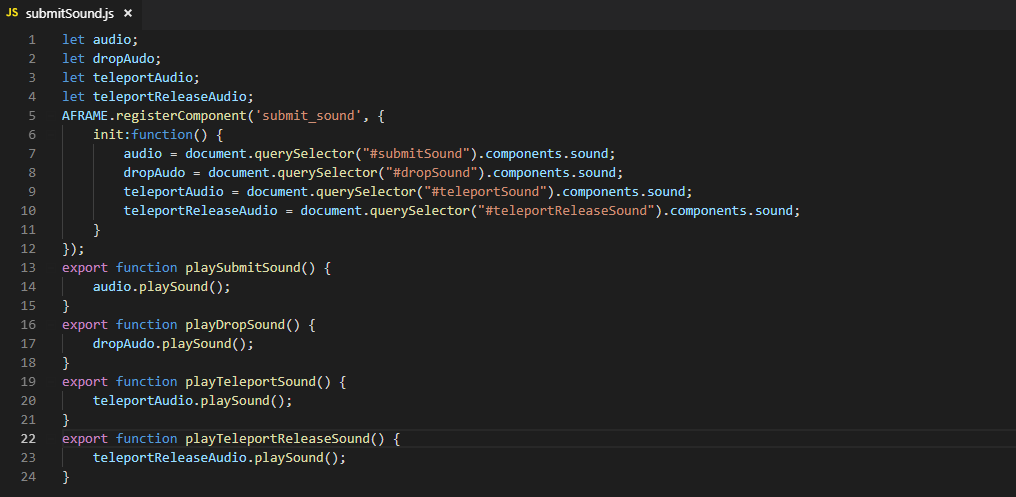
\includegraphics[width=\textwidth]{images/submitSound.png}
\begin{lstlisting}[language=JavaScript, style=htmlcssjs]
let audio;
AFRAME.registerComponent('submit_sound', {
    init:function() {
        audio = document.querySelector("#submitSound").components.sound;
    }
});
export function playSubmitSound() {
    audio.playSound();
}
\end{lstlisting}
\label{fig:submitSound} 
\end{figure}
 
 \subsection{Arbeitsoberflächendesinfektion auf der Vive}
 Das Feedback der Desinfektion der Arbeitsoberfläche wird durch eine Hinweis-Box über dem Mülleimer und zwei versteckten Umschaltern auf der Arbeitsoberfläche implementiert.
 
 Solange ein Desinfektionstuch in Hder and gehalten wird, wird eine rote Hinweis-Box über dem Mülleimer dargestellt, um die Botschaft zu vermitteln, dass das Tuch und Handschuhe in den Mülleimer eingeworfen werden sollen, aber nicht zu der Zeit, wo die Voraussetzung (Desinfektion der Arbeitsoberfläche) noch nicht erfüllt wird.
 
 Gleichzeitig überprüfen die zwei Umschalter alle 0.5 Sekunden, ob die Kollision zwischen dem Tuch und dem Umschalter erkannt wird. Wenn ein Schalter das Tuch getroffen hat, wird der entsprechende Zustand für den Vive Controller als {\fontfamily{qcr}\selectfont true} gesetzt.
 
 Solange die beiden Zustände der Umschalter {\fontfamily{qcr}\selectfont true} sind, wechselt die Farbe der Hinweis-Box über dem Mülleimer zu grün, um die Information zu teilen, dass das Tuch und die Handschuhe in den Mülleimer eingeworfen werden dürfen.
 
 image: m5 Arbeitsfläche desinfektion Szene .........
 
 \subsection{Animation}
 Die Animation in A-Frame wird auch durch ein HTML Element {\fontfamily{qcr}\selectfont a-animation} bezeichnet. Das übergeordnete Element ist das Objekt das zu animieren ist. Die genaue Manipulation wird durch die Attribute des {\fontfamily{qcr}\selectfont a-animation} Elements konfiguriert. (Tabelle ~\ref{tab:aAnimation})
 
\begin{table}
\centering
\caption{Wichtige Attribute von a-animation Element}
\begin{tabular}{lll} 
\toprule
Name      & Beschreibung                                                                                                          & Standard- \\
& & einstellung  \\
attribute & Das Attribut des übergeordneten Elements zu animieren                                                                 & rotation             \\
begin     & Name des Events, die Animation aufzurufen                                                                             & ''                   \\
from      & Die Wert am Anfang                                                                                                    &                      \\
to        & Die Wert am Ende                                                                                                      &                      \\
dur       & Die Zeitdauer der Animation                                                                                           & 1000                 \\
direction & Die Richtung der Animation (zwischen Anfang und Ende)                                                                  & normal               \\
fill      & \begin{tabular}[c]{@{}l@{}}Der Effekt der Animation zu bestimmen, \\wenn die Animation deaktiviert wird.\end{tabular} & forwards             \\
repeat    & Die Zahl der Wiederholung der Animation                                                                               & 0                    \\
easing    & Die Erleichterung der Animation                                                                                       & ease                 \\
\bottomrule
\end{tabular}
\label{tab:aAnimation} 
\end{table}
 
 Um die Animation einfach zu benutzen, wird eine Funktion entwickelt. Das \glqq a-animation\grqq Element wird erstellt. Und nach dem Laufen der Animation wird das Element nach dem Bedarf, der als Parameter eingegeben, entworfen oder behalten. (Abbildung ~\ref{fig:aAnimation})
 
\begin{figure}[ht]
\vspace*{1em}
\centering
\caption[Animation]{Animation}
%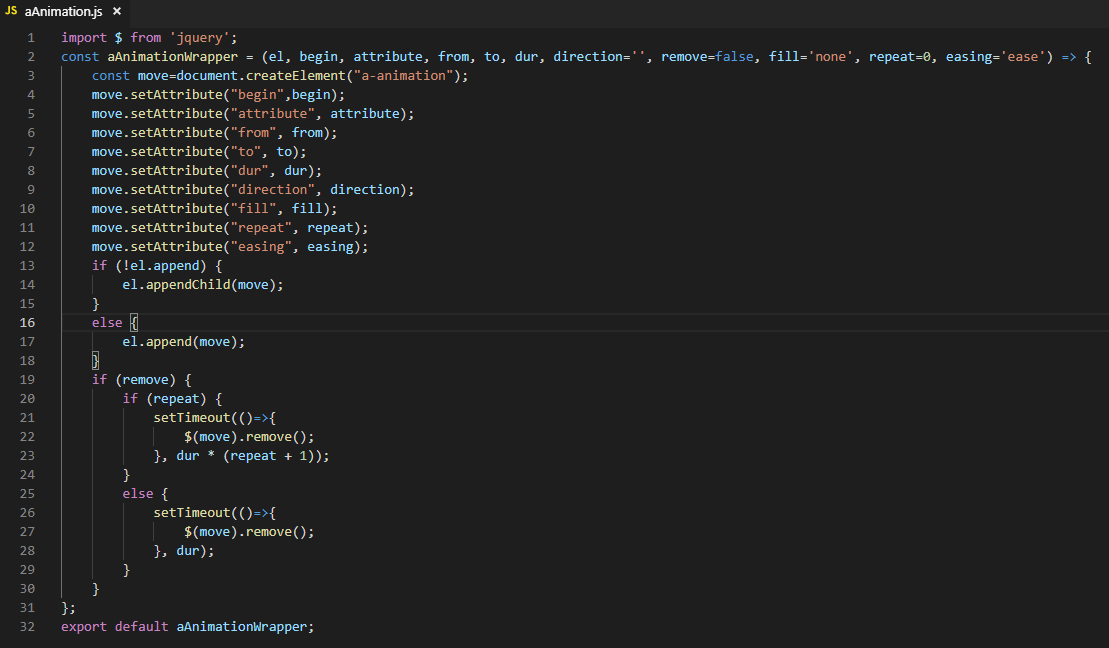
\includegraphics[width=\textwidth]{images/aAnimation.png}
\begin{lstlisting}[language=JavaScript, style=htmlcssjs]
import $ from 'jquery';
const aAnimationWrapper = (el, begin, attribute, from, to,
    dur, direction='', remove=false, fill='none',
    repeat=0, easing='ease') 
    => {
    const move=document.createElement("a-animation");
    move.setAttribute("begin",begin);
    move.setAttribute("attribute", attribute);
    move.setAttribute("from", from);
    // set other attributes here ...
    if (!el.append) {
        el.appendChild(move);
    }
    else {
        el.append(move);
    }
    if (remove) {
        if (repeat) {
            setTimeout(()=>{
                $(move).remove();
            }, dur * (repeat + 1));
        }
        else {
            setTimeout(()=>{
                $(move).remove();
            }, dur);
        }
    }
};
export default aAnimationWrapper;
\end{lstlisting}
\label{fig:aAnimation} 
\end{figure}
 
 \subsection{Hand}
 
 Durch das {\fontfamily{qcr}\selectfont a-animation} Element kann das ganze Objekt animiert werden. Um kompliziertere Animationen zu realisieren, wird das Objekt während der Modellierung direkt animiert.
 
 Das Hand Modell wird in Blender animiert. Zuerst wird das Skelett für die Hand erstellt. Mit der Funktion \glqq Set Parent To \grqq\ können das Modell und die Skelett zusammen verbinden. Durch \glqq Key Frame\grqq\ kann die Hand animiert werden. (Abbildung ~\ref{fig:handSetParentTo} \& Abbildung ~\ref{fig:handKeyframes})
 
\begin{figure}[ht]
\vspace*{1em}
\centering
\caption[Verbinden Modell und Skelett]{Verbinden Modell und Skelett}
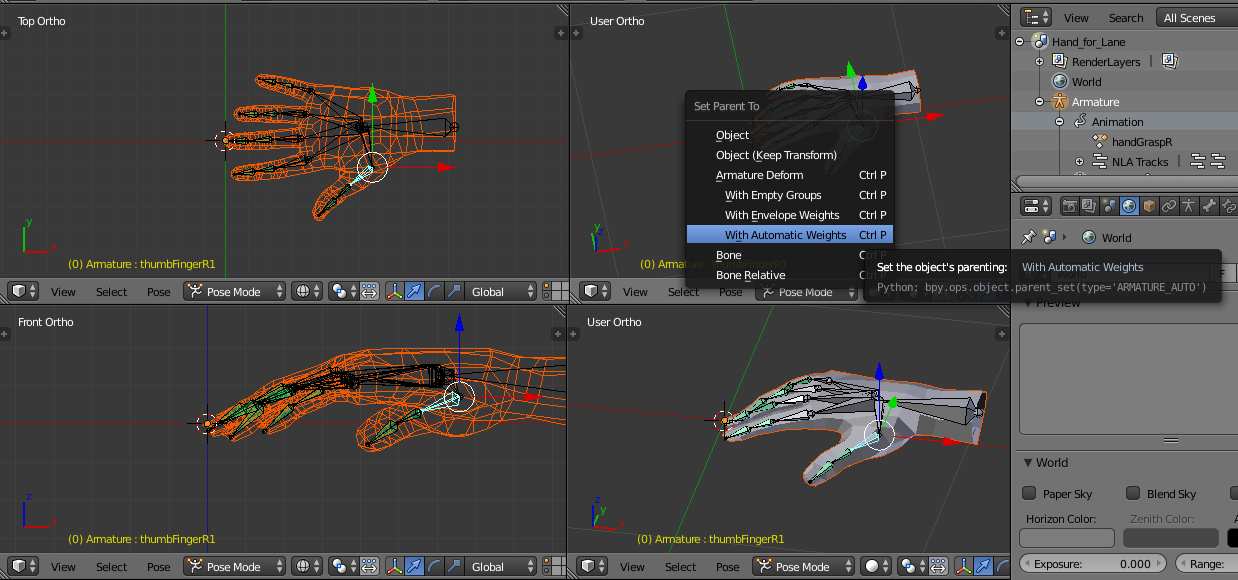
\includegraphics[width=\textwidth]{images/handSetParentTo.png}
\label{fig:handSetParentTo} 
\end{figure}

\begin{figure}[ht]
\vspace*{1em}
\centering
\caption[Einstellung der Animation von Hand]{Einstellung der Animation von Hand}
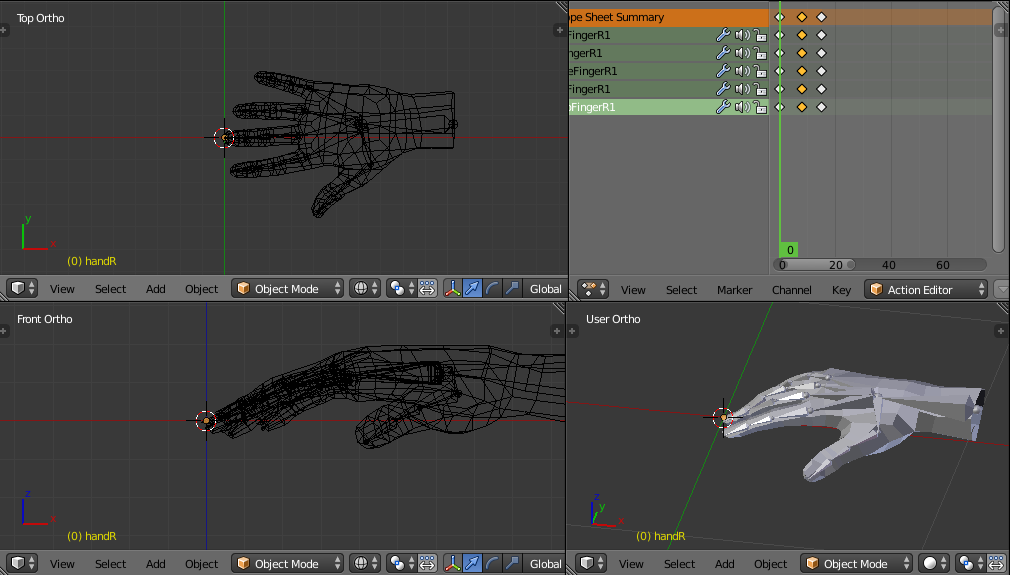
\includegraphics[width=\textwidth]{images/handKeyframes.png}
\label{fig:handKeyframes} 
\end{figure}
 
 Das Modell wird als glTF 2.0 exportiert. Das glTF 2.0 ist ein Format für 3D Objekte, die für webbasierte Applikation entwickelt wurde. Die Vorteile sind die kleine Größe und die Unterstützung der Animation.
 
 Bei A-Frame kann die Animation durch das Attribut {\fontfamily{qcr}\selectfont animation-mixer} (Abbildung ~\ref{fig:handAnimation}) von dem Hand Modell aufgerufen werden. Allerdings kann der Zeitraum der Animation bei A-Frame nicht ausgewählt werden, was mit Unity oder Unreal Engine geschafft werden kann. Deshalb kann der Effekt, dass die Hand leicht eine Faust macht während des Drucks auf dem Hair-Trigger und die Hand eine Faust macht während der Auslösung auf den Hair-Trigger lockert, nicht implementiert werden.
 
\begin{figure}[ht]
\vspace*{1em}
\centering
\caption[Aufruf der Animation von Hand]{Aufruf der Animation von Hand}
%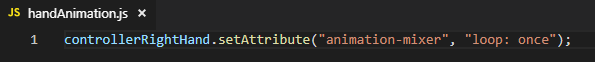
\includegraphics[width=\textwidth]{images/handAnimation.png}
\begin{lstlisting}[language=JavaScript, style=htmlcssjs]
controllerRightHand.setAttribute("animation-mixer", "loop: once");
\end{lstlisting}
\label{fig:handAnimation} 
\end{figure}
 
 \subsection{Uhr}
 
 Die Uhr hat zwei Funktionen in der Szene, die Uhrzeit darzustellen und die 30 Sekunden Markierung während der Händedesinfektion zu zeigen.
 
 \subsubsection{Uhrzeit darstellen}
 
 Um die reale Uhrzeit darzustellen, wird eine Klasse {\fontfamily{qcr}\selectfont clock\_hand\_roll} entwickelt. Da sich der Zeiger jede Sekunde bewegt, wird die built-in Funktion {\fontfamily{qcr}\selectfont tick} benutzt. Die von {\fontfamily{qcr}\selectfont tick} aufgerufenen Funktionen werden jede Sekunde ein Mal durchgeführt, wie {\fontfamily{qcr}\selectfont setInterval}.
 
 Mit der Hilfe der Funktion {\fontfamily{qcr}\selectfont tick} wird jede Sekunde das Attribut {\fontfamily{qcr}\selectfont Rotation} aller drei Zeiger aktualisiert. 
 
 Um den Winkel der Rotation zu berechnen wird zuerst die aktuelle Uhrzeit durch die Klasse {\fontfamily{qcr}\selectfont Data} erhalten. Und mit den Funktionen {\fontfamily{qcr}\selectfont getSeconds}, {\fontfamily{qcr}\selectfont getMinutes}, {\fontfamily{qcr}\selectfont getHours} werden die Ziffern für jeden Zeiger berechnet.
 
 Danach wird der Winkel jedes Zeigers berechnet, der sich bei jeder Bewegung dreht. Für Sekundenzeiger und Minutenzeiger ist der Winkel {\fontfamily{qcr}\selectfont  360/60}. Für Stundenzeiger ist der Winkel {\fontfamily{qcr}\selectfont  360/12}.
 
 Das Produkt von der Ziffer mal entsprechendem Winkel bei jeder Bewegung ist der Winkel der Rotation auf der X-Ebene in den Koordinate. (Abbildung ~\ref{fig:clockRoll})
 
\begin{figure}[ht]
\vspace*{1em}
\centering
\caption[Drehung des Zeigers der Uhr]{Drehung des Zeigers der Uhr}
%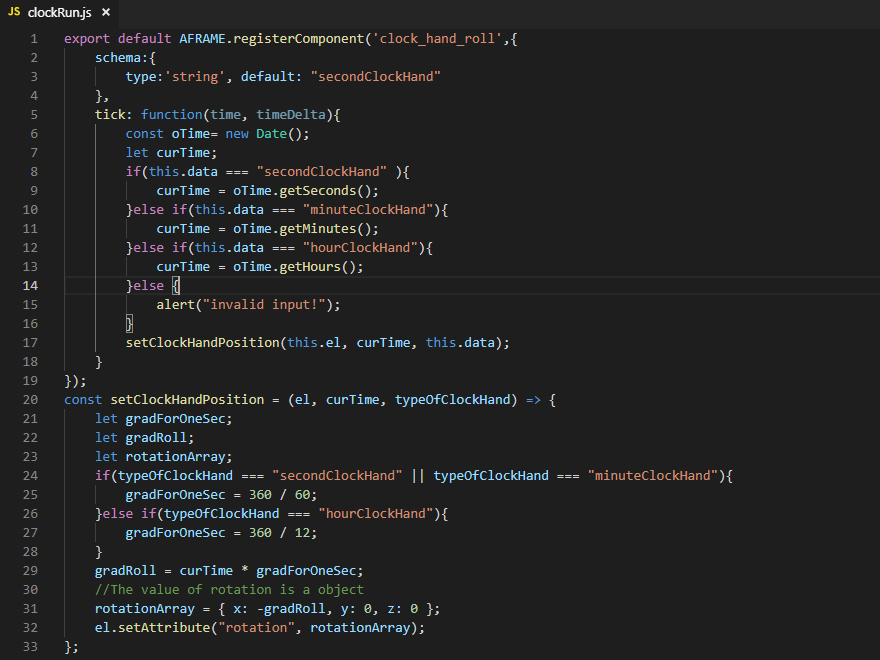
\includegraphics[width=\textwidth]{images/clockRoll.png}
\begin{lstlisting}[language=JavaScript, style=htmlcssjs]
export default AFRAME.registerComponent('clock_hand_roll',{
    schema:{
        type:'string', default: "secondClockHand"
    },
    tick: function(time, timeDelta){
        const oTime= new Date();
        let curTime;
        if(this.data === "secondClockHand" ){
            curTime = oTime.getSeconds();
        }else if(this.data === "minuteClockHand"){
            curTime = oTime.getMinutes();
        }else if(this.data === "hourClockHand"){
            curTime = oTime.getHours();
        }else {
            alert("invalid input!");
        }
        setClockHandPosition(this.el, curTime, this.data);
    }
});
const setClockHandPosition = (el, curTime, typeOfClockHand) => {
    let gradForOneSec;
    let gradRoll;
    let rotationArray;
    if(typeOfClockHand === "secondClockHand" || typeOfClockHand === "minuteClockHand"){
        gradForOneSec = 360 / 60;
    }else if(typeOfClockHand === "hourClockHand"){
        gradForOneSec = 360 / 12;
    }
    gradRoll = curTime * gradForOneSec;
    //The value of rotation is a object
    rotationArray = { x: -gradRoll, y: 0, z: 0 };
    el.setAttribute("rotation", rotationArray);
};
\end{lstlisting}
\label{fig:clockRoll} 
\end{figure}
 
 \subsubsection{30 Sekunden Markierung}
 Solange der Griff des Händedesinfektionsspenders gedrückt wird, wird ein Event {\fontfamily{qcr}\selectfont  handwashing} emittiert. Danach wird ein A-Frame Element {\fontfamily{qcr}\selectfont  a-gltf-model} für die 30 Sekunden Markierung mit entsprechenden Attributen erstellt. Die Methode, die Rotation zu errechnen, ist die gleiche, wie die Methode für den Sekundenzeiger. Nach 30 Sekunden wird die Markierung des Element entworfen. (Abbildung ~\ref{fig:clockMarker})
 
\begin{figure}[ht]
\vspace*{1em}
\centering
\caption[Markierung der Uhr]{Markierung der Uhr}
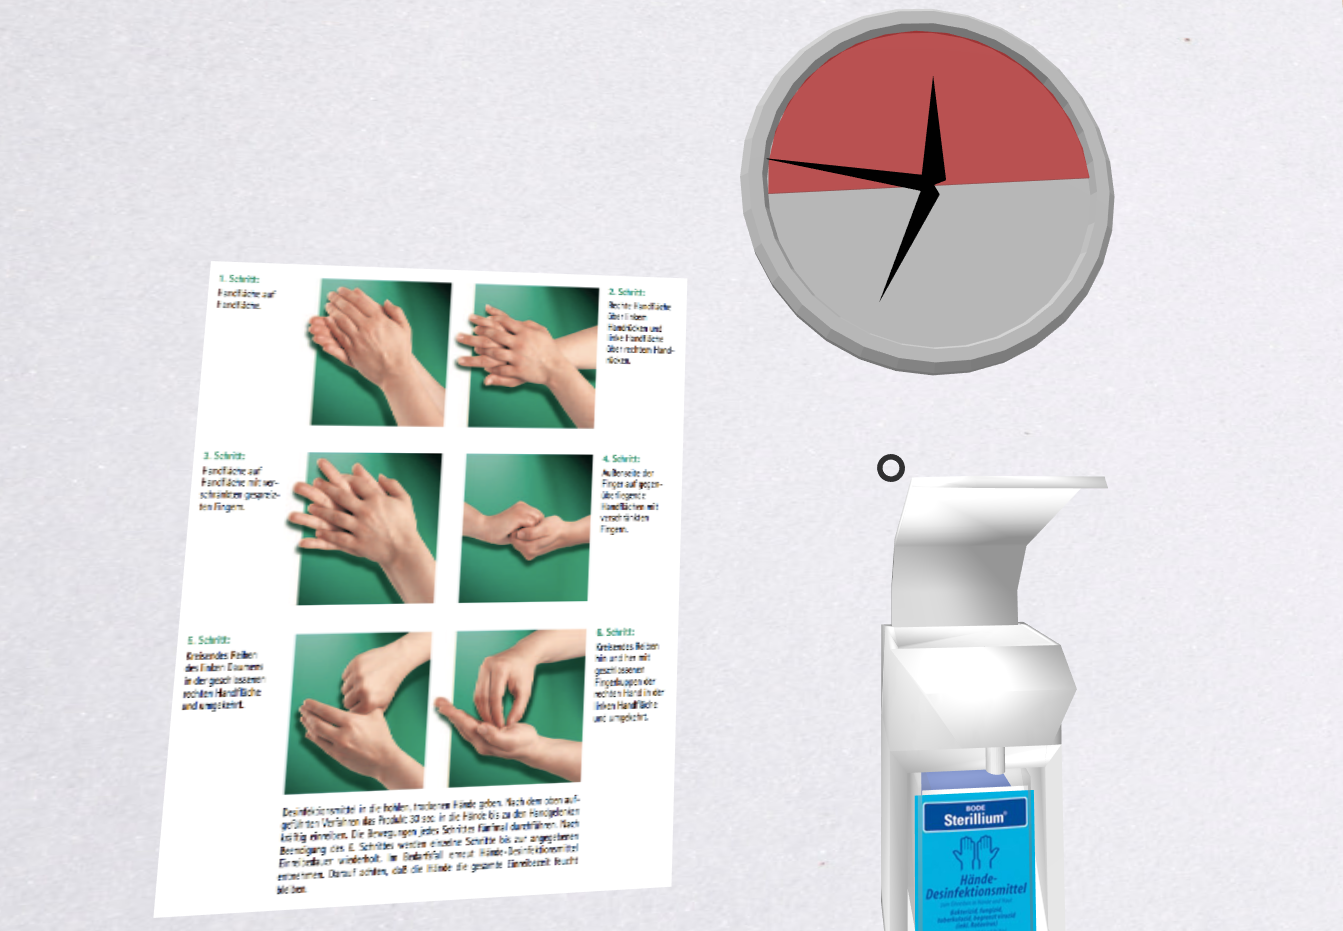
\includegraphics[width=\textwidth]{images/clockMarker.png}
\label{fig:clockMarker} 
\end{figure}

\section{Zusammenfassung}
Das Projekt wird in zwei Teilen implementiert, die Gestaltung des Unterrichts in LMS und die Entwicklung der WebVR Applikation.

Wegen des Mangels der fachlichen Kenntnissen werden die meisten Materialien aus dem Internet verwendet. Allerdings ist das Ziel, das LMS und die WebVR Applikation zu verbinden, erreichtet.

Als Schwerpunkt des Projektes wird die meiste Zeit in die WebVR Applikation investiert. Die Implementierung wird iterativ verbessert und ergänzt. Obwohl nicht alle Funktionen optimal implementiert sind, wird die Konzeption der cross-platformen WebVR Applikation realisiert.
